% !TEX program = xelatex
\documentclass[UTF8,a4paper,12pt]{ctexart}
\usepackage{geometry}
\geometry{left=2.5cm,right=2.5cm,top=2.5cm,bottom=2.5cm}
\usepackage{amsmath,amssymb,bm}
\usepackage{graphicx}
\usepackage{booktabs,array,multirow}
\usepackage{subcaption}
\usepackage{enumitem}
\usepackage{float}
\usepackage{hyperref}
\hypersetup{hidelinks}
\graphicspath{{exp3_images/}}
\newcommand{\blank}[1][2.5cm]{\mbox{\underline{\hspace{#1}}}}
\newcommand{\answer}{\par\noindent\textbf{填写：}\blank[0.86\textwidth]\par}
\numberwithin{equation}{section}

\title{《动态数字图像相关法实验》实验报告}
\author{姓名\blank[2.5cm] \quad 学号\blank[3cm] \quad 同组成员\blank[4cm]\\[1em]
实验地点\blank[3cm] \quad 实验日期\blank[4cm]}
\date{}
\begin{document}
\maketitle
\tableofcontents
\clearpage

\section{实验目的}
\begin{enumerate}
  \item 掌握数字图像相关法的基本原理，以及三维数字图像相关法测量物体表面位移场的方法和技术。
  \item 了解三维数字图像相关系统的使用方法。
  \item 熟悉采用动态数字图像相关法研究结构动态响应问题的实验装置及其有关的试验技术。
  \item 了解铝板动态响应的特点。
\end{enumerate}

\section{实验装置、仪器及器材}
\begin{enumerate}
  \item 三维动态光学应变测量系统（两台 FASTCAM SA-Z PHOTRON LIMITED 480K-M-16GB 高速相机、采集卡、GOM Correlate Professional 2017 软件、Photron FASTCAM Viewer 软件）。
  \item 标定板（MV200，尺寸 $250\times200\,\mathrm{mm}^2$）。
  \item 激振器（Mini Shaker，Type 4810）。
  \item 功率放大器（Bruel \& Kjaer，Power Amplifier，Type 2718）。
  \item 信号发生器（RIGOL，DG1022，2 Channel，20 MHz，100 MSa/s）。
  \item 光源（两个，dedocool）。
  \item 铝板（尺寸 $150.0\times246.5\times2.0\,\mathrm{mm}^3$）。
  \item DELL 笔记本电脑。
\end{enumerate}

\section{实验内容}
本实验测试对象为一个铝板，其尺寸为 $150.0\times246.5\times2.0\,\mathrm{mm}^3$。
\begin{enumerate}
  \item 掌握三维动态光学应变测量系统的使用方法。
  \item 针对铝板，采用激振器进行不同频率下的稳态激励，测试表面离面位移场随时间变化的分布。
  \item 截取多个截面的表面位移场分布图，进行结构动态响应特征分析。
  \item 从铝板表面提取多个测点的位移随时间变化曲线，进行结构局部动态响应特点分析。
\end{enumerate}

\section{实验测量原理、方法与测量过程}
\subsection{动态三维数字图像相关方法测量结构动态响应的基本原理}
三维数字图像相关法（DIC）的实验装置和光路如图\ref{fig:exp3-dic-system}所示。当白光照射到涂有散斑斑点的试件表面时，表面的散斑会随着试件变形而变化。通过相机拍摄试件变形过程中的散斑图变化进行变形跟踪，进而反演出试件表面的实际变形。由左、右两个相机可以得到两个不同视角的试件表面散斑图像，通过测量图像之间的视差可以计算出试件表面的三维形貌，实现立体摄影测量。

\begin{figure}[H]
  \centering
  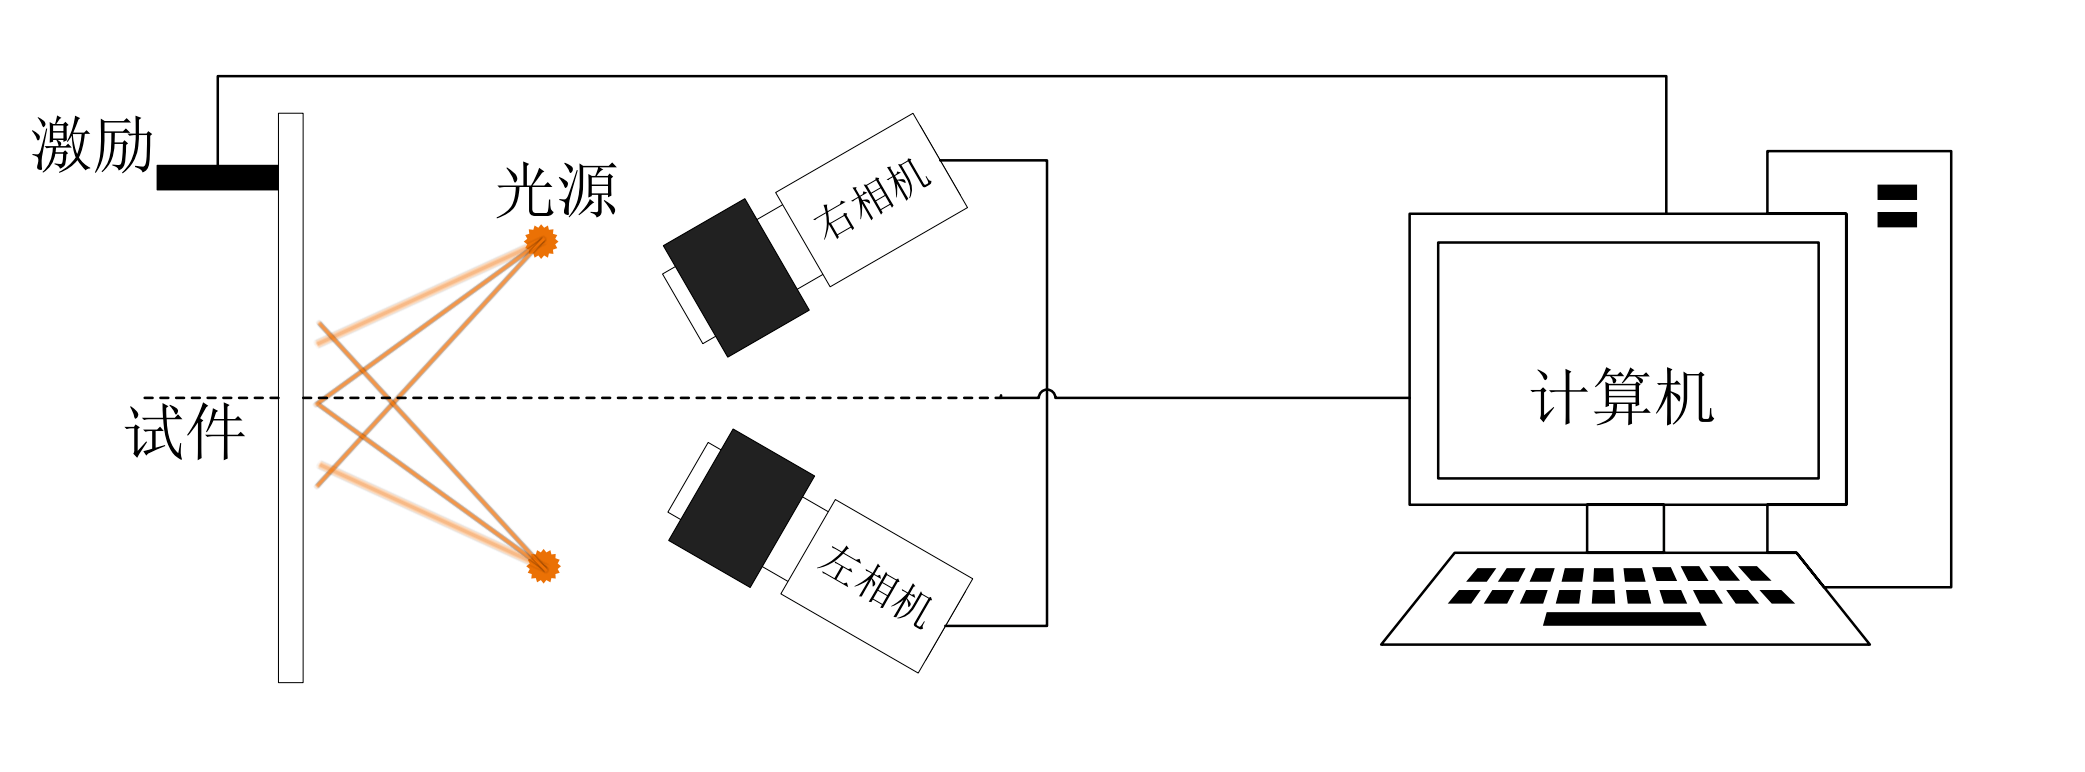
\includegraphics[width=0.72\textwidth]{p03_img01.png}
  \caption{三维数字图像相关法的实验装置}
  \label{fig:exp3-dic-system}
\end{figure}

三维数字图像相关法的实验首先需要进行立体系统建模和标定：计算光线的交点，并保证光线必须处在相同坐标系中，如图\ref{fig:exp3-calibration-principle}所示。

\begin{figure}[H]
  \centering
  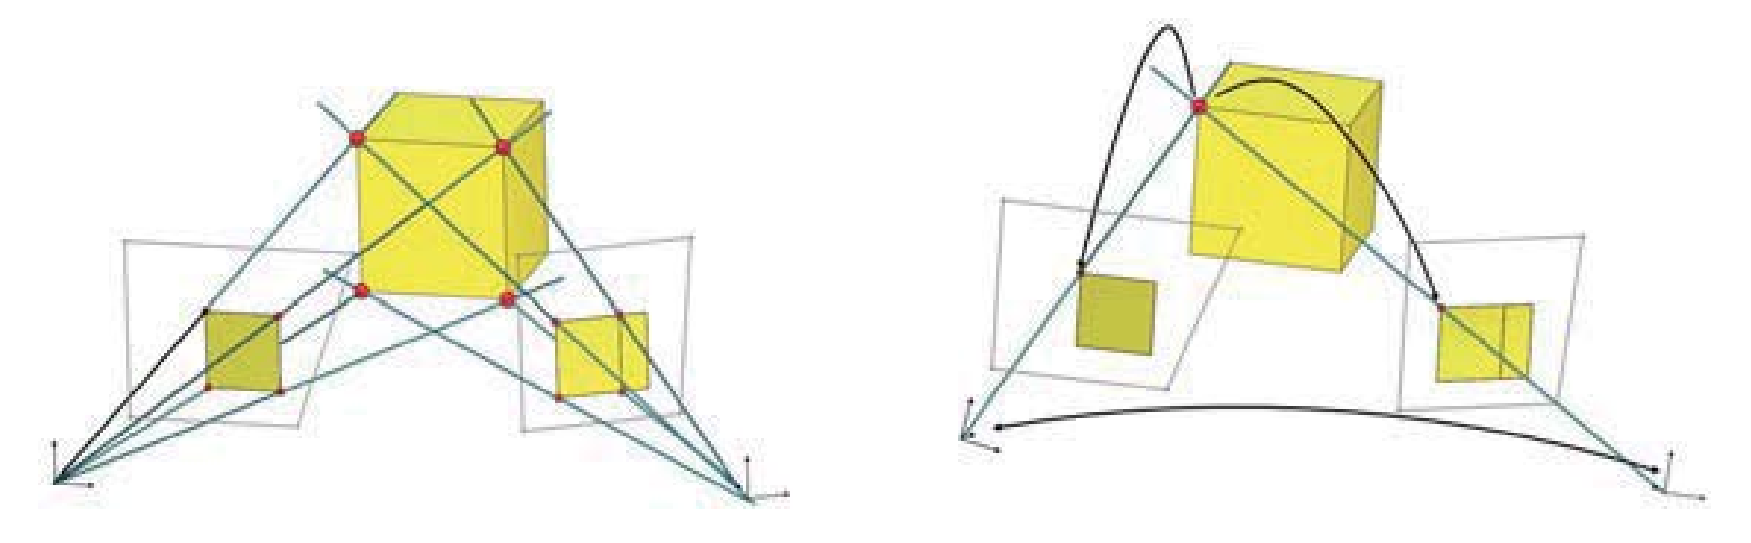
\includegraphics[width=0.6\textwidth]{p03_img02.png}
  \caption{立体摄影标定}
  \label{fig:exp3-calibration-principle}
\end{figure}

对于二维 DIC，变形前后的两幅散斑图存在相关性。通过分析变形前后的散斑图，可以得到散斑沿面内 $x$ 和 $y$ 方向的相对位移，即物体沿横向和纵向的相对变形 $(u,v)$。如图\ref{fig:exp3-speckle}所示，设 $(x,y)$ 是变形前的一点，$(x',y')$ 是变形后的相应点，则两者关系为
\begin{subequations}
\begin{align}
  x'&=x+u+\Delta x\frac{\partial u}{\partial x}+\Delta y\frac{\partial u}{\partial y},\\
  y'&=y+v+\Delta x\frac{\partial v}{\partial x}+\Delta y\frac{\partial v}{\partial y}.
\end{align}
\end{subequations}

\begin{figure}[H]
  \centering
  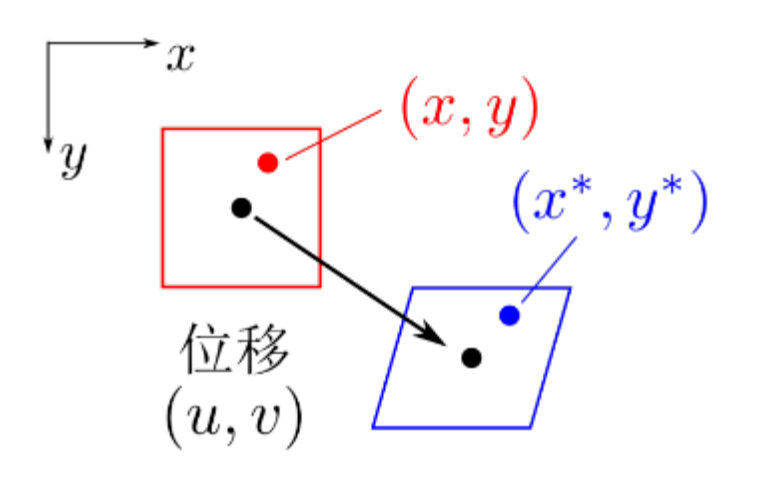
\includegraphics[width=0.32\textwidth]{p04_img01.png}
  \caption{变形前后散斑点对应图}
  \label{fig:exp3-speckle}
\end{figure}

若用函数 $f(x_i,y_i)$ 表示变形前某一点 $(x_i,y_i)$ 处的灰度值，$g(x'_i,y'_i)$ 表示变形后对应点 $(x'_i,y'_i)$ 处的灰度值，则两者的相关系数为
\begin{equation}
  C=\frac{\sum_{i=1}^{m_s}\sum_{j=1}^{m_s}
  [f(x_i,y_i)-\bar{f}][g(x'_i,y'_i)-\bar{g}]}
  {\sqrt{\sum_{i=1}^{m_s}\sum_{j=1}^{m_s}[f(x_i,y_i)-\bar{f}]^2}
  \sqrt{\sum_{i=1}^{m_s}\sum_{j=1}^{m_s}[g(x'_i,y'_i)-\bar{g}]^2}}.
\end{equation}
其中 $\bar{f}$ 和 $\bar{g}$ 分别为变形前后子区灰度的平均值。$0\le C\le1$；$C=1$ 时两者完全相关，$C=0$ 时两者完全不相关。只要两者相关，则以位移为变量的相关函数 $C(u,v)$ 曲面为一单峰曲面。当位移 $u$ 和 $v$ 分别固定时，$C$ 则为正态分布曲线。

由于点 $(x,y)$ 的像素值不具有唯一性，所以以该点为中心选定一定邻域范围内的像素值集合形成子区并进行匹配，使子区内各像素在变形前后图像中的对应灰度值最接近，如图\ref{fig:exp3-subset}所示。三维 DIC 方法的位移测量算法与二维 DIC 类似，但是每个点需要进行 3 次 DIC 计算，如图\ref{fig:exp3-3d-dic}所示。

\begin{figure}[H]
  \centering
  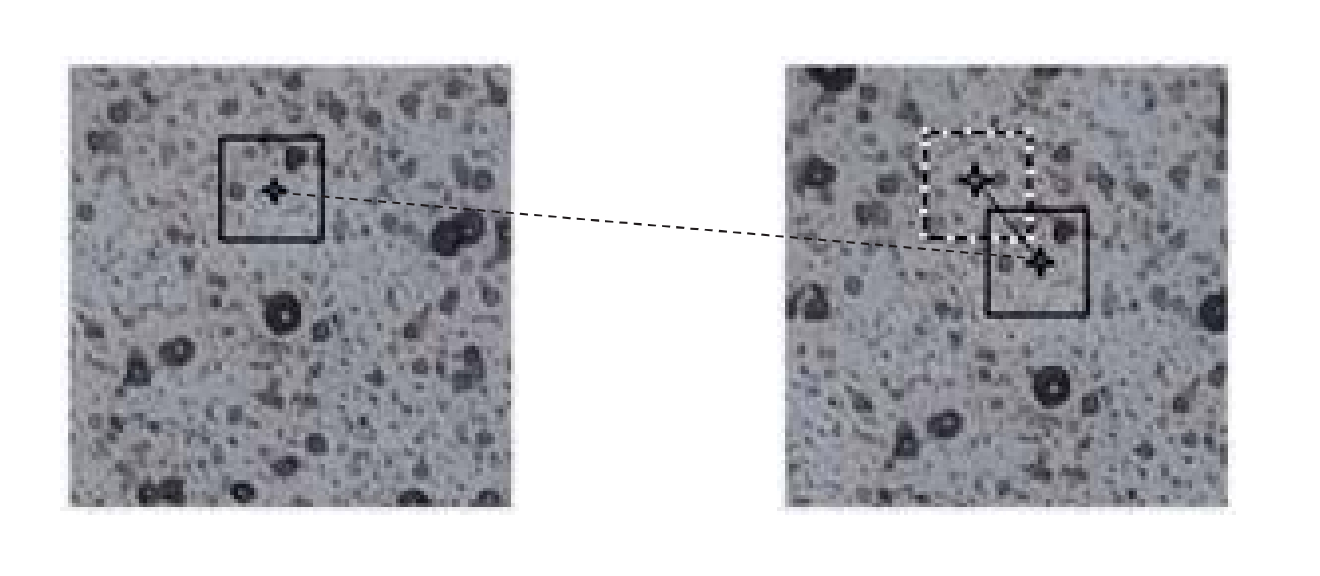
\includegraphics[width=0.45\textwidth]{p04_img02.png}
  \caption{子区的匹配}
  \label{fig:exp3-subset}
\end{figure}

\begin{figure}[H]
  \centering
  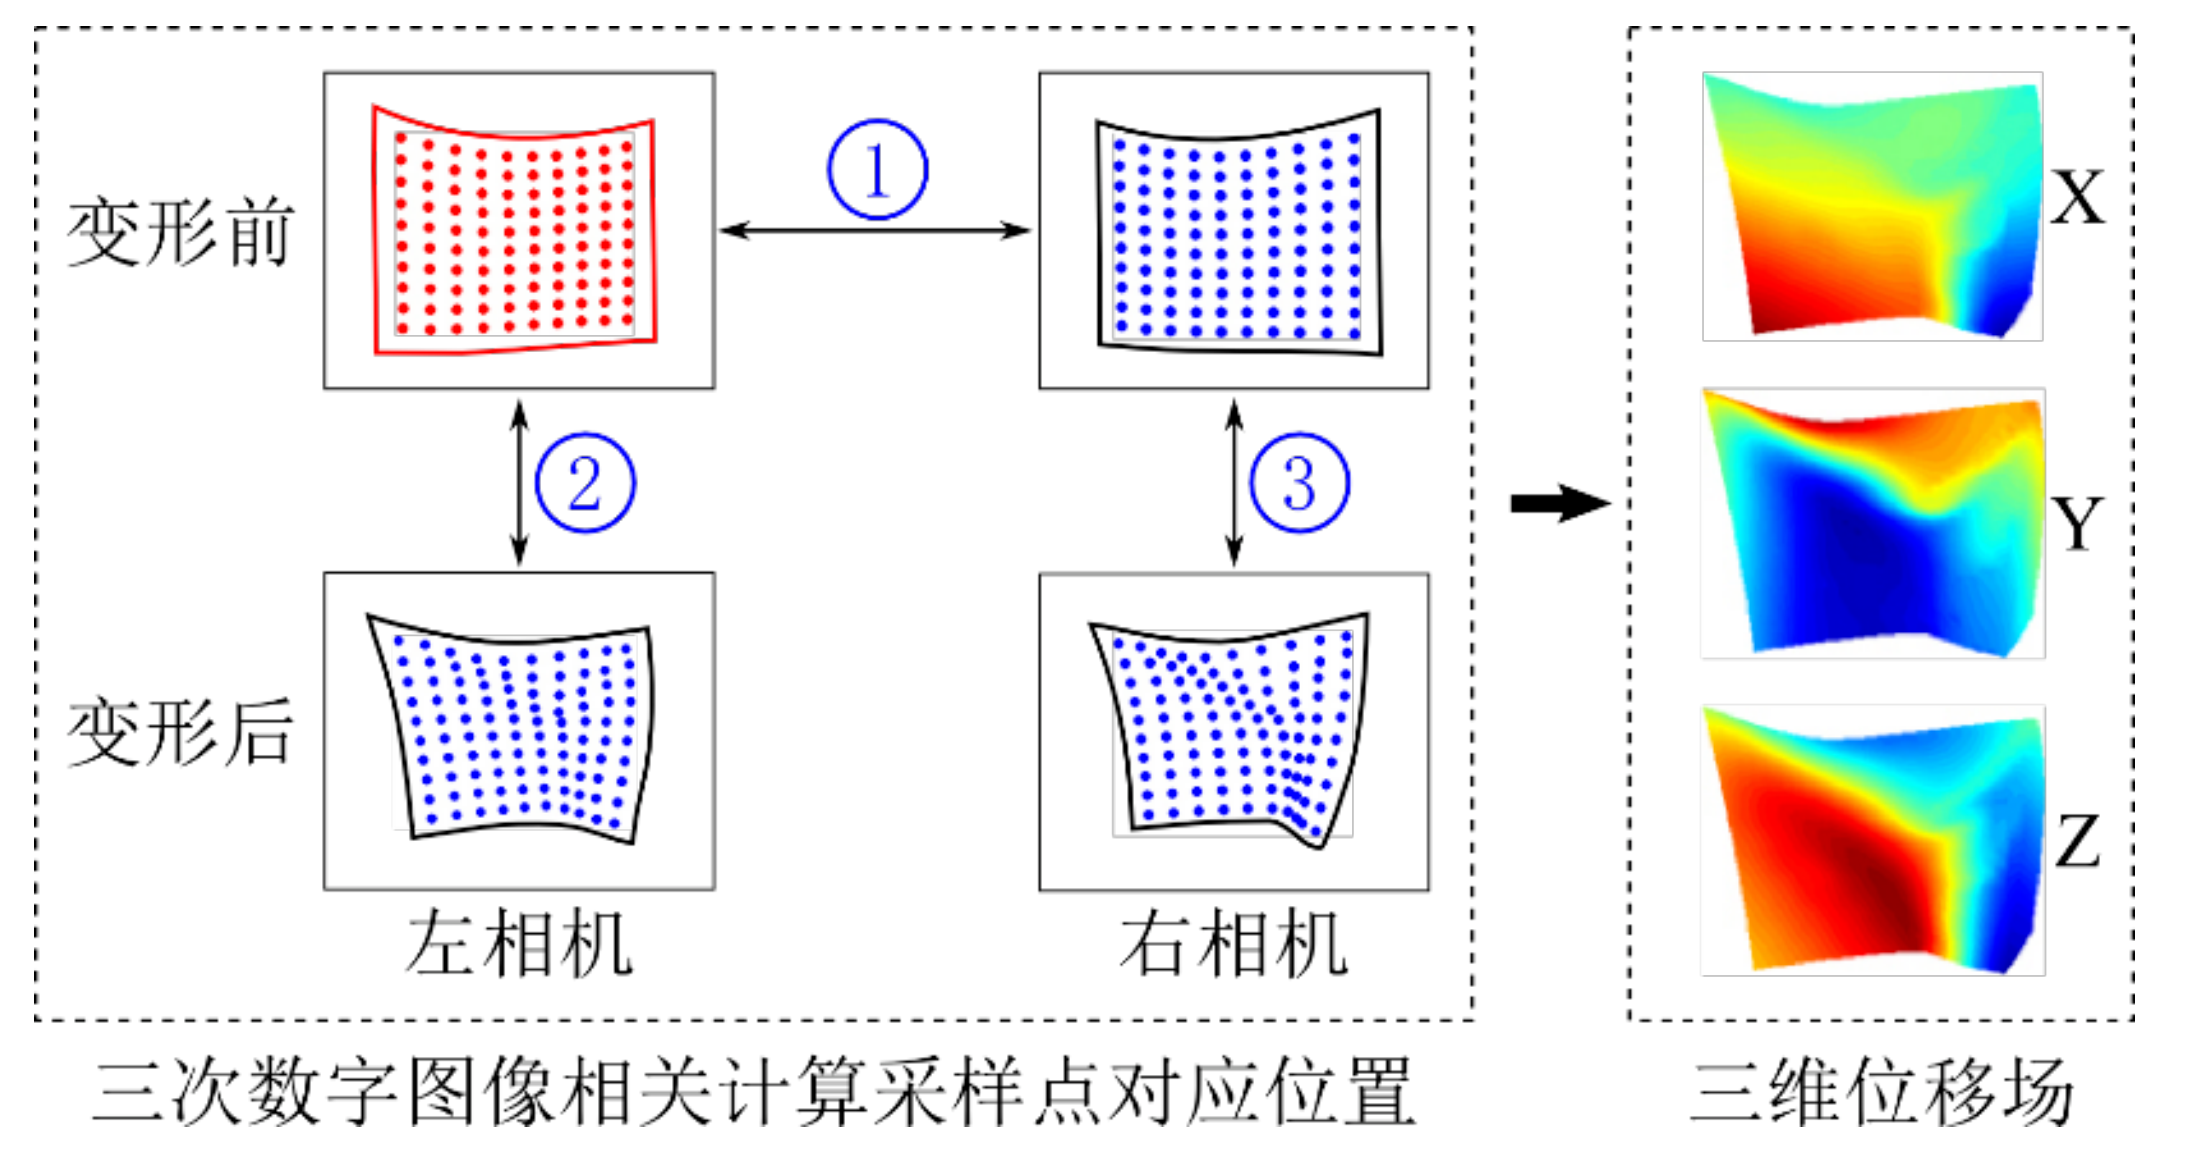
\includegraphics[width=0.68\textwidth]{p04_img03.png}
  \caption{三维 DIC 位移场计算}
  \label{fig:exp3-3d-dic}
\end{figure}

\subsection{动态测量过程}
\subsubsection{高速摄影系统的安装和设置}
\begin{enumerate}[label=\alph*)]
  \item 高速摄影系统的固定与数据线连接：三脚架立于试件前方，固定左右相机于支架上，通过 Netgear 开关把两个相机连接到笔记本电脑。
  \item 启动高速摄影系统：打开左右高速相机电源，预热相机 10 分钟。笔记本电脑关闭防火墙，禁用无线网络。确保系统连接成功，检查 Netgear 网线接口是否灯亮和网络本地连接是否启用并处于“未识别的网络”状态。双击 PFV（Photron FASTCAM Viewer）软件图标，启动高速摄影软件。
  \item 配置立体相机同步系统：左相机为主相机，右相机为从相机，左侧相机给右侧相机提供触发及同步信号。将 PFV 切换到 LIVE 模式，选择主相机 Camera No.1，点击 Camera Option，在弹窗里选择 I/O，并将 GENERAL OUT 1 设置为 SYNC POS；选择从相机 Camera No.2，点击 Camera Option，在弹窗中选择 I/O，并将 SYNC IN 设置为 ON CAM POS。在 PFV 软件实时视图里查看是否为右侧相机启用了 E-Sync，由此保证两个相机的同步性能。
\end{enumerate}

\subsubsection{相机标定}
选择 $250\times200\,\mathrm{mm}^2$ 标定板 MV200，调节两个相机的夹角为 $25^\circ$--$35^\circ$。
\begin{enumerate}[label=\alph*)]
  \item 在整个标定过程中，两个相机选用全屏模式（最大相机分辨率），精度 Revolution 选择 $1024\times1024$。
  \item 曝光调节：点击快门（Shutter），曝光时长选择为 $1/38095$ s。
  \item 触发模式设置：在相机菜单里点击 Trigger Mode，选择 Random，设置记录数量为 1，使每遥控触发一次只摄取一幅图像。
  \item 聚焦调节：点击鼠标右键，选择 Cursor，点击 Show 调出十字光标；再次点击鼠标右键，选择 Cursor，点击 Lock at Central all view，将左右十字光标都定在各自视窗中心。通过移动三脚架和相机滑轨，调整双相机与试件的角度和距离，始终保持左右相机视图的十字中心处于待测物表面同一位置。
  \item 标定图像：按图\ref{fig:exp3-calibration-poses}指定的标定板 13 个不同方向拍摄 13 幅图像，然后将标定图像输入 GOM Correlate Professional 软件进行标定评估。通过调整到合适位置，记录相机靠近标定板时的位置刻度\blank[1.8cm]、远离标定板时的位置刻度\blank[1.8cm]，以及测量体积中心点时的位置刻度\blank[1.8cm]。
  \item 具体标定操作：在相机菜单 LIVE（实时）模式里点击 Record（记录），界面切换为 Trigger In（触发）。按图\ref{fig:exp3-calibration-poses}调整标定板位置，每次通过按击遥控按键（或点击 Trigger In）控制图像记录，PFV 软件记录左右相机各一幅图像。记录完 13 幅标定图像后，点击 Rec Done（记录完成）结束记录过程。
  \item 保存标定图像：记录完成后，PFV 软件自动切换到 SAVE（保存）模式。检查记录的 0 到 12（共 13 幅图像）是否完整。点击 Save 进行标定图像转存，在弹出窗口中选择 tiff 格式和 Option 图像分辨率 8 bit。
\end{enumerate}

\begin{figure}[H]
  \centering
  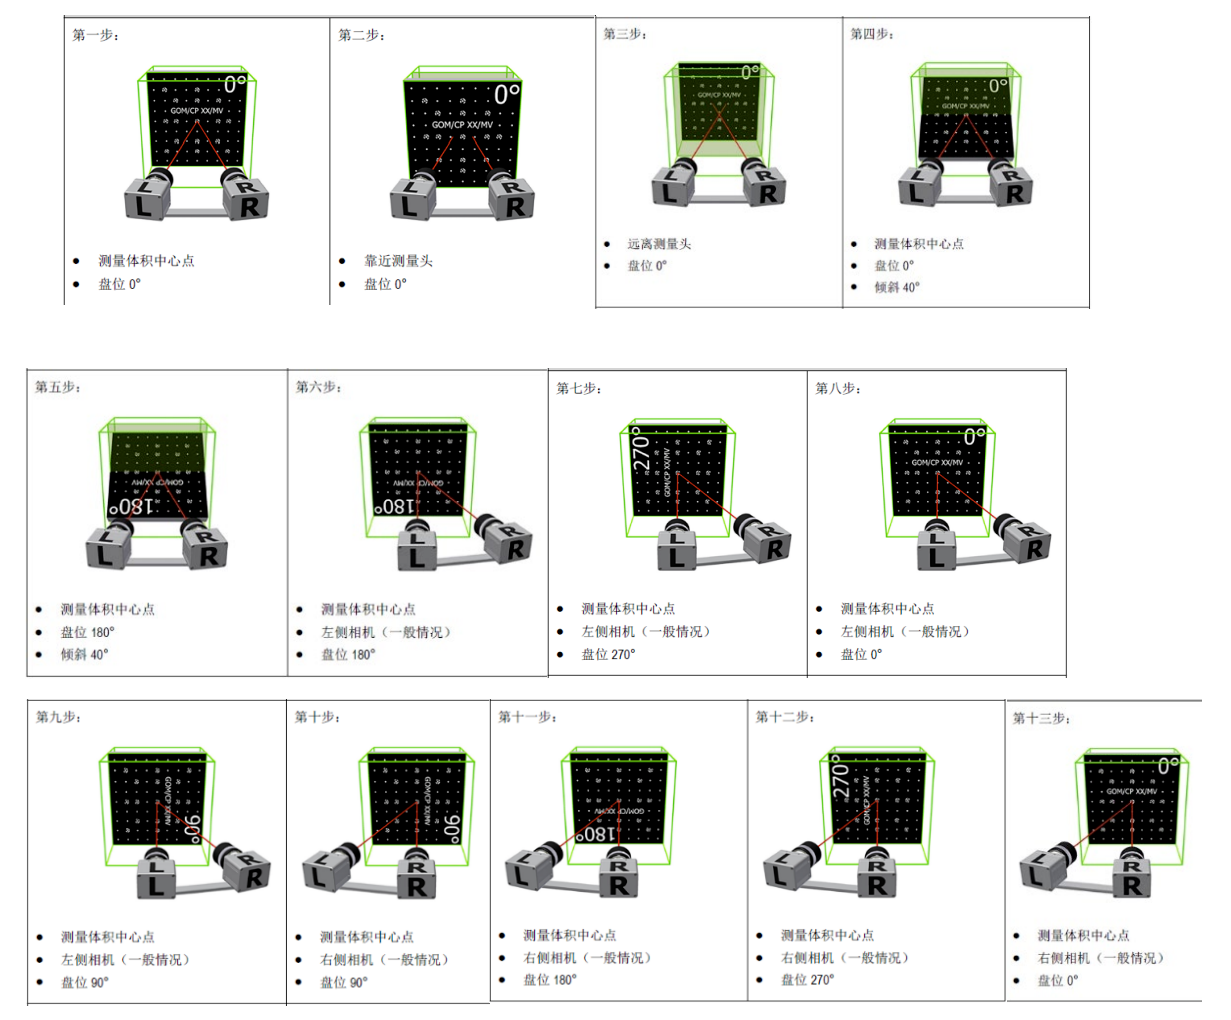
\includegraphics[width=0.78\textwidth]{p06_img01.png}
  \caption{标定图的拍摄方位}
  \label{fig:exp3-calibration-poses}
\end{figure}

\subsubsection{实验测试}
\begin{enumerate}[label=\alph*)]
  \item 把试件在加载装置上固定好。试件采用一边固定、三边自由的边界约束方式，动态外载荷由激振器激励，由三维数字图像相关系统采集图像。
  \item 点击鼠标右键，选择 Cross Cursor，点击 Central at all view，调出中央十字光标，调整双相机与试件的角度和距离，使左右相机视图的十字中心处于试件表面同一位置。
  \item 调节左右光源投射角度，使被测区域光强明亮均匀。
  \item 选择触发模式，在 Trigger Mode 里选择 Start 触发模式，记录触发后的图像。
  \item 在 Frame Rate 里选择合适的图像采集频率。
  \item 在 Shutter 里选择合适的曝光时间，使散斑黑白分明。
  \item 在 PFV 相机菜单 Live 模式里点击 Record，按键转为 Trigger In 等待触发状态。检查系统，若无问题，点击 Trigger In 进行图像采集。界面显示图像数量持续增加，待相机内存被填满后自动结束图像采集。点击 Rec Done 结束记录过程，PFV 软件自动切换到 Save 模式，按同样的操作保存图像。
\end{enumerate}

\subsubsection{图像处理与结果输出}
\begin{enumerate}[label=\alph*)]
  \item 动态实验测试标定计算：打开 GOM Correlate Professional 软件，创建项目，导入 Photron 相机记录的标定图像并用软件进行标定计算。
  \item 试件表面变形分析：使用功能输入三维图像系列，将使用外部三维立体相机系统拍摄的图像输入 GOM 软件。首先选择“曲面成分”，选择要分析的曲面区域，之后定义合适的坐标系。选择需要的截面或者点，将 Z 坐标的数值从针对固定值改为针对参考阶段，选择合适的参考时间，以保证位移曲线的对称性。
  \item 结果输出：输出选择截面与选择点的位移坐标等信息。
\end{enumerate}

\subsection{实验测试内容}
\begin{enumerate}
  \item 激励 23 Hz，功率放大器 2 V，采样频率 500 Hz，曝光时长 $1/38095$ s。
  \item 激励 151 Hz，功率放大器 2.5 V，采样频率 3000 Hz，曝光时长 $1/30769$ s。
\end{enumerate}

\section{实验测量结果分析与讨论}
\noindent\textbf{使用说明：}以下结果图从原报告提取，用于保留图件和版式。写作时请用同名文件替换为本组云图和位移曲线，并根据本组结果修改分析。

针对每种激励方式，选取不同截面及测量点的动态响应进行分析。在相同实验参数条件下，考虑两个相差半个周期的时刻，对其振动状态进行比较。

\subsection{标定结果}
标定过程中，采样频率设置为 500 Hz，曝光时间为 $1/38095$ s。实验标定结果如图\ref{fig:exp3-calibration-result}所示。

\begin{figure}[H]
  \centering
  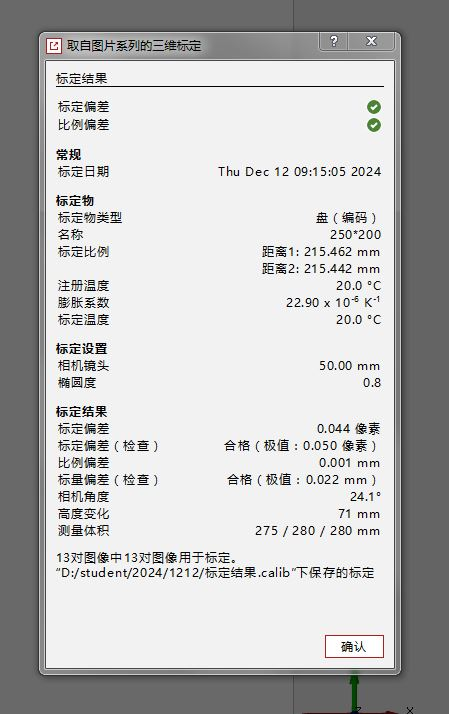
\includegraphics[width=0.38\textwidth]{p07_img01.jpeg}
  \caption{实验标定结果}
  \label{fig:exp3-calibration-result}
\end{figure}
\noindent 标定偏差及标定是否成功的判断：\blank[0.62\textwidth]

\subsection{截面动态响应特征分析}
\subsubsection{一阶模态分析（23 Hz 激励）}
考虑两个相差半个周期的时刻，并通过位移云图进行展示，如图\ref{fig:exp3-mode1-cloud}所示。为便于比较，两个云图采用相同标度的颜色条。

\begin{figure}[H]
\centering
\subcaptionbox{时刻1}[0.47\textwidth]{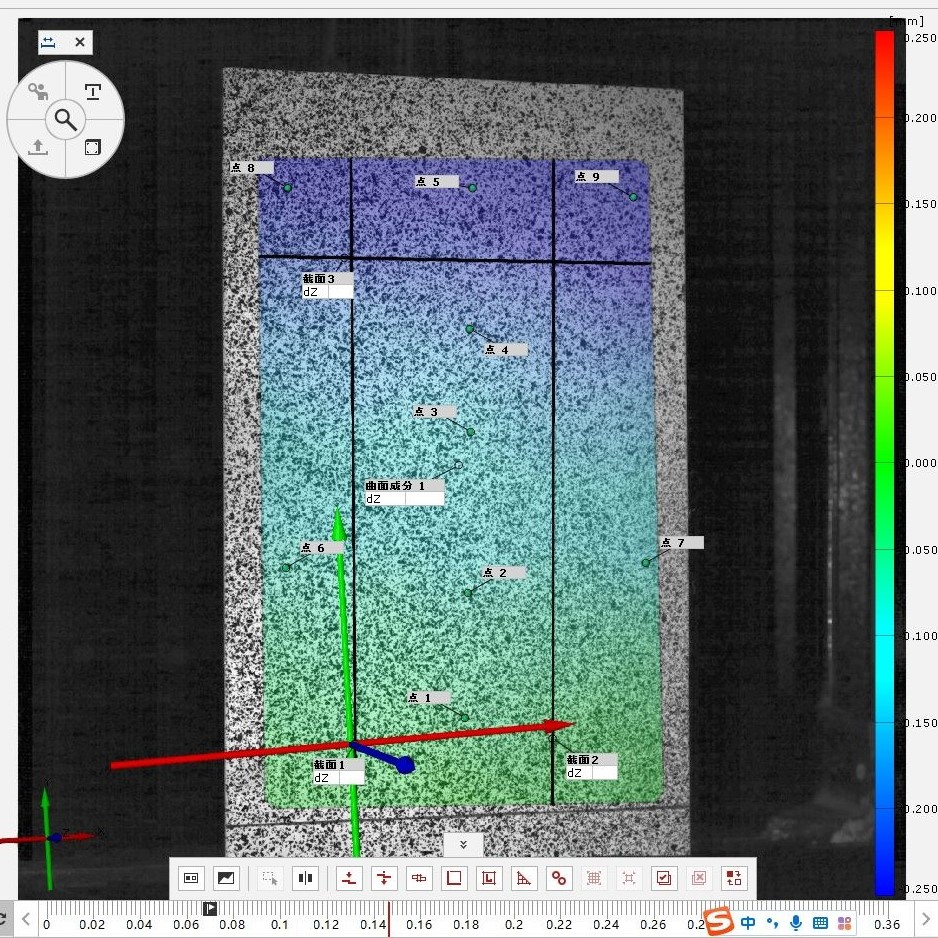
\includegraphics[width=\linewidth]{p08_img01.jpeg}}\hfill
\subcaptionbox{时刻2}[0.47\textwidth]{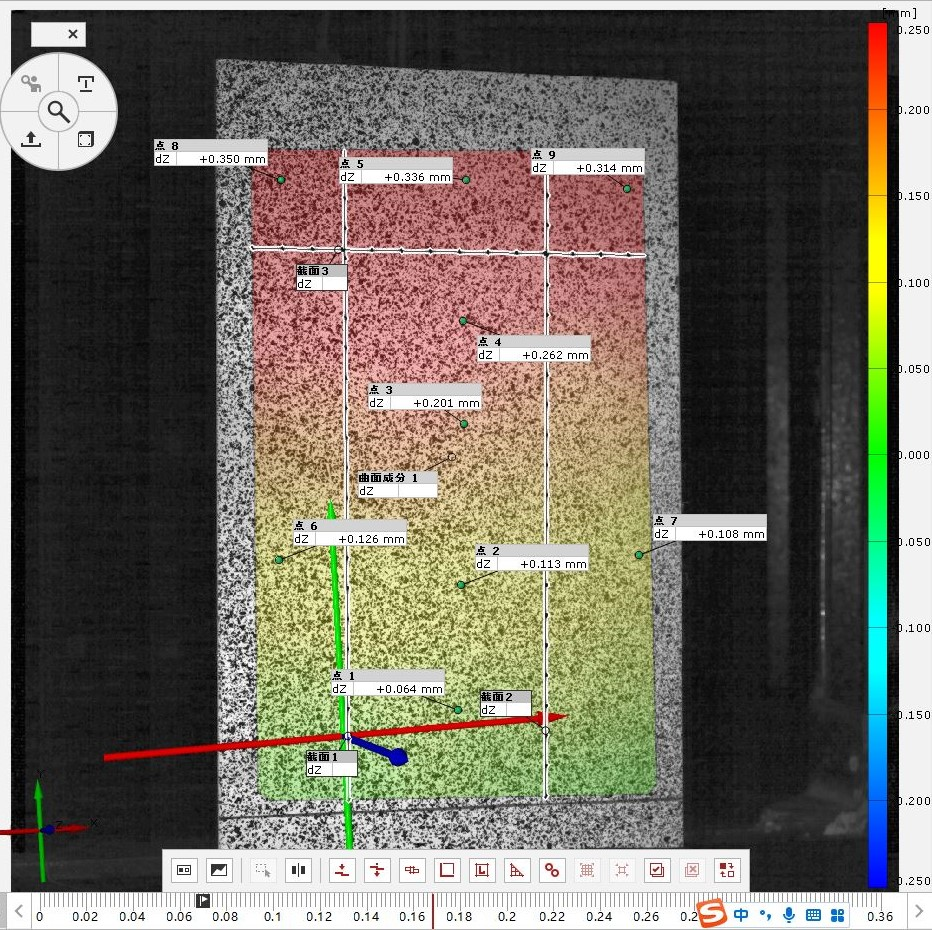
\includegraphics[width=\linewidth]{p08_img02.jpeg}}
\caption{一阶模态云图}
\label{fig:exp3-mode1-cloud}
\end{figure}

在图中选取三个截面，提取其沿 $z$ 坐标方向的位移信息，结果如图\ref{fig:exp3-mode1-section}所示。截面 1 与截面 2 沿纵向分布，可用于观察弯曲模态；截面 3 沿横向分布，可用于展示潜在的扭转模态。

\begin{figure}[H]
  \centering
  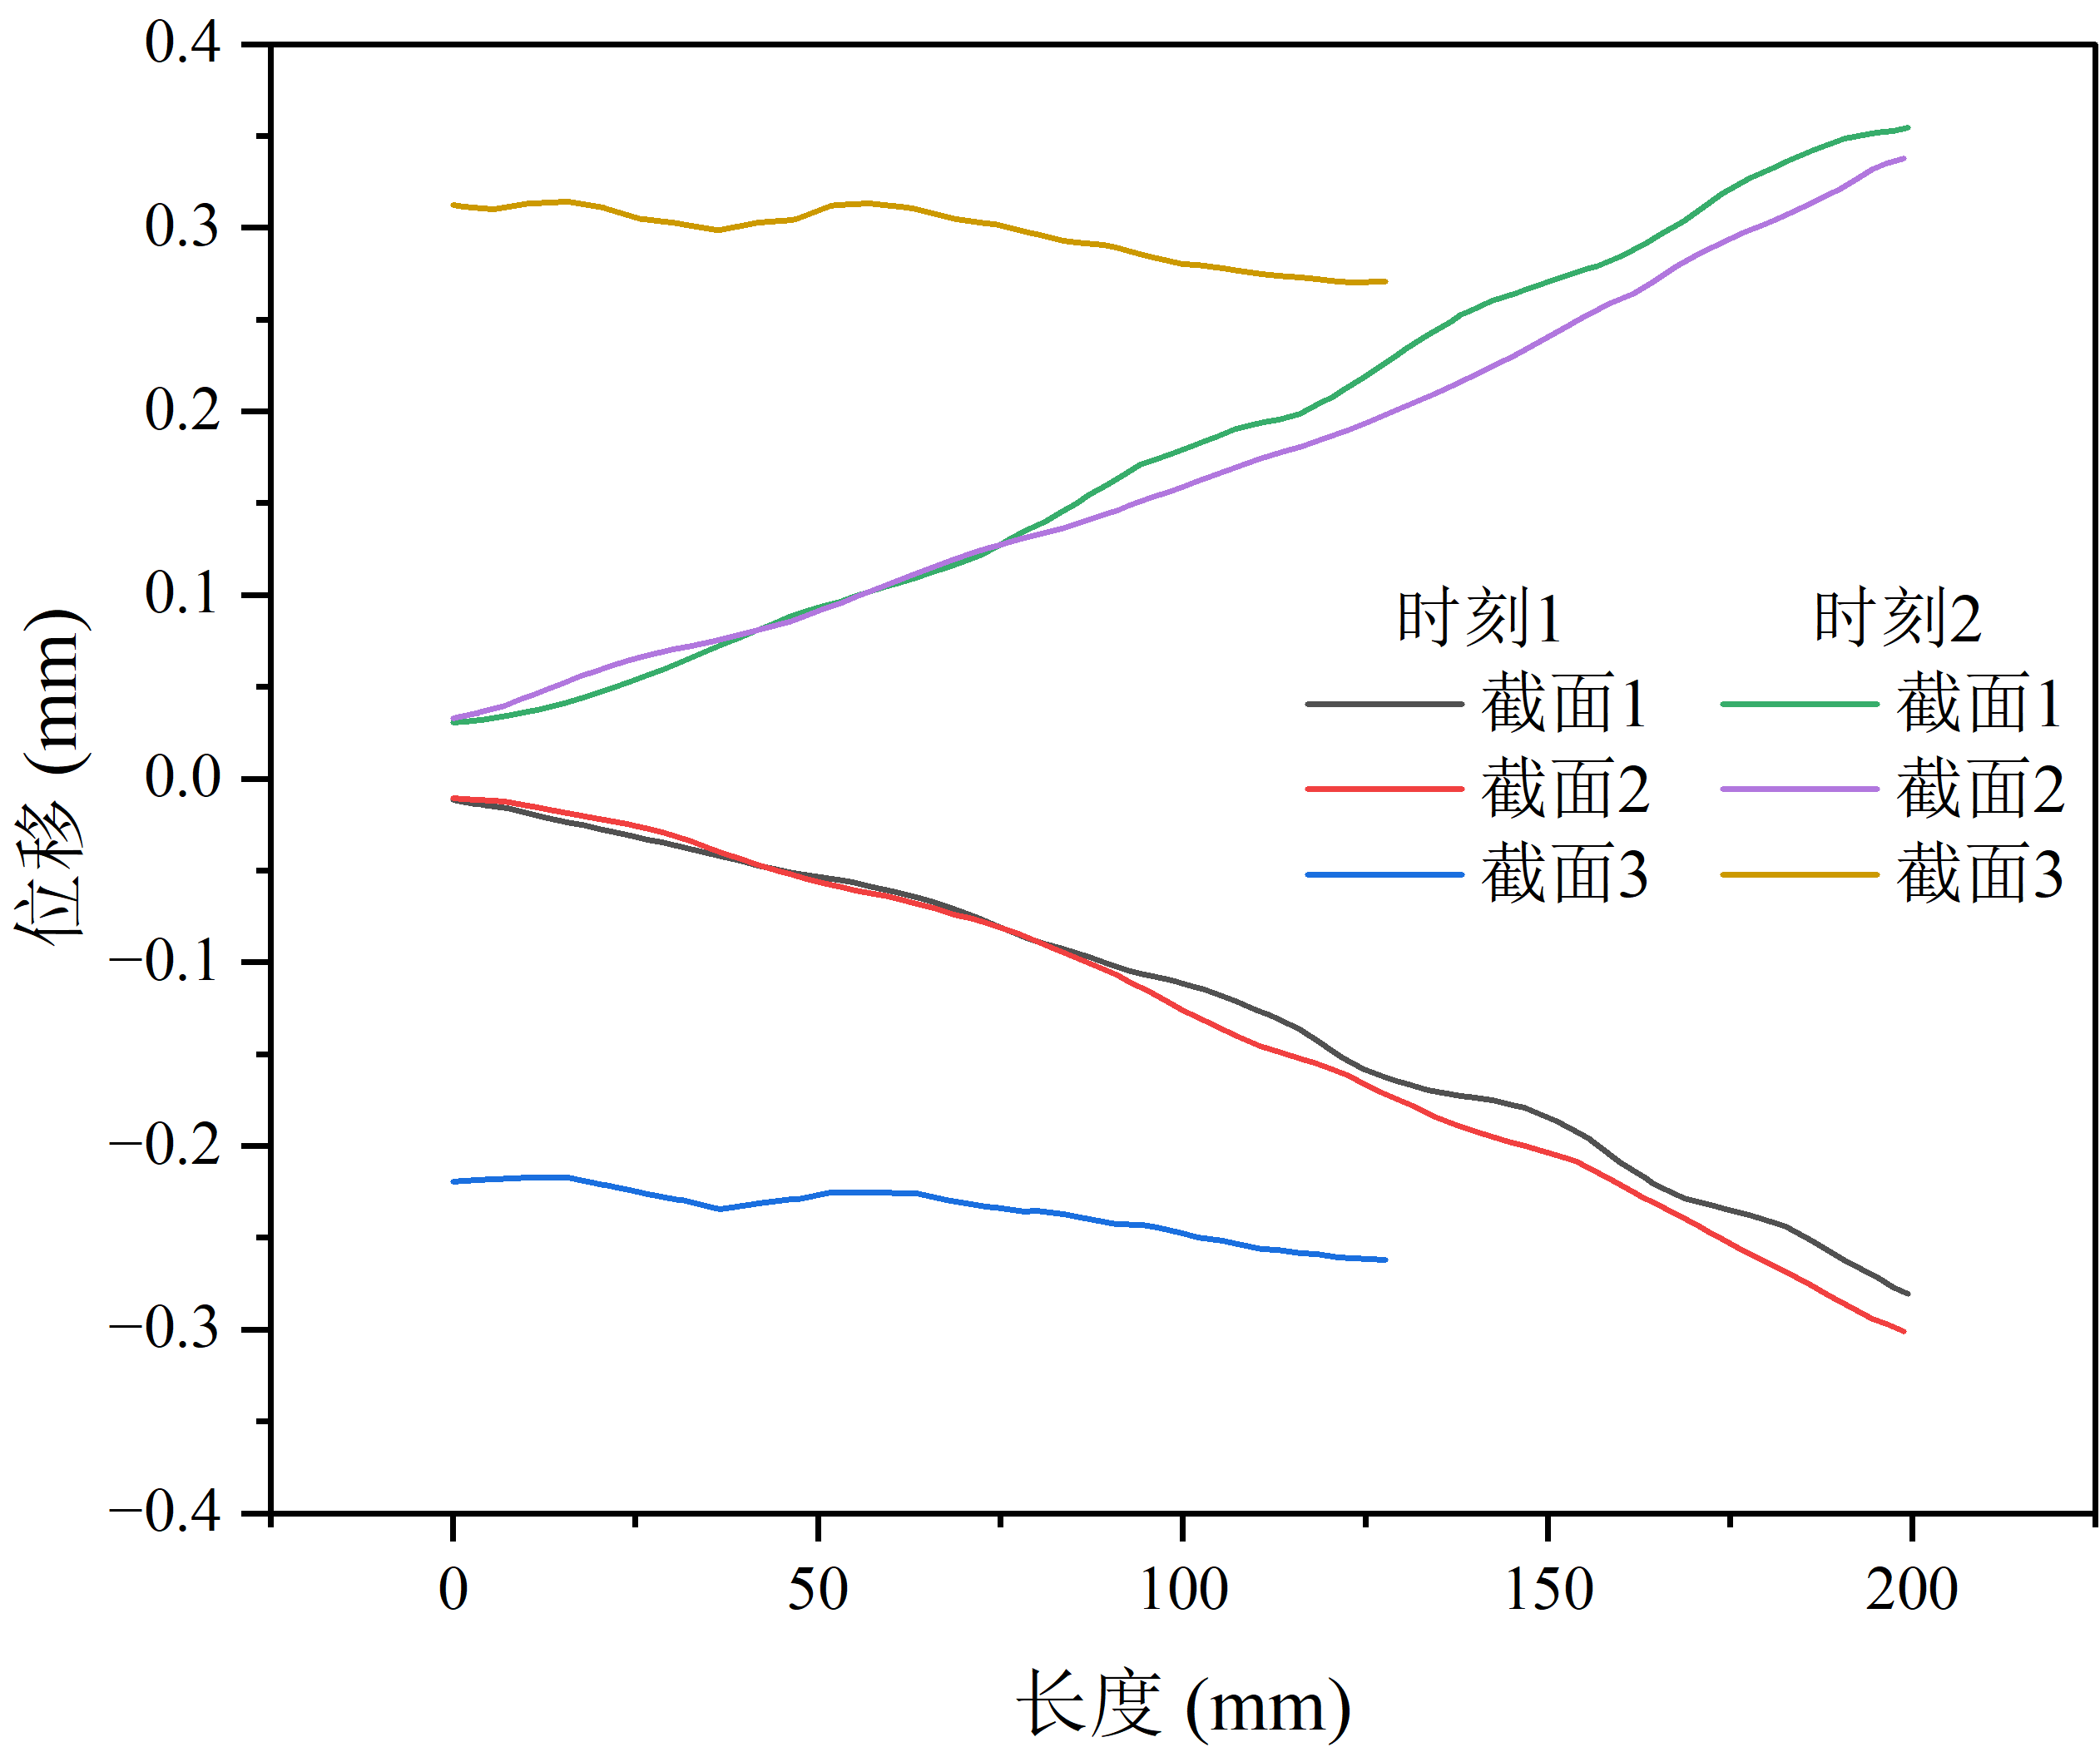
\includegraphics[width=0.66\textwidth]{p08_img03.png}
  \caption{一阶模态选取截面位移图}
  \label{fig:exp3-mode1-section}
\end{figure}
分析一端固支铝板的一阶模态形态、各截面位移曲线的异同，以及是否存在明显扭转。
\answer

\subsubsection{二阶模态分析（151 Hz 激励）}
同样考虑两个相差半个周期的时刻，并通过位移云图展示，如图\ref{fig:exp3-mode2-cloud}所示。两个云图采用相同标度的颜色条。

\begin{figure}[H]
\centering
\subcaptionbox{时刻1}[0.47\textwidth]{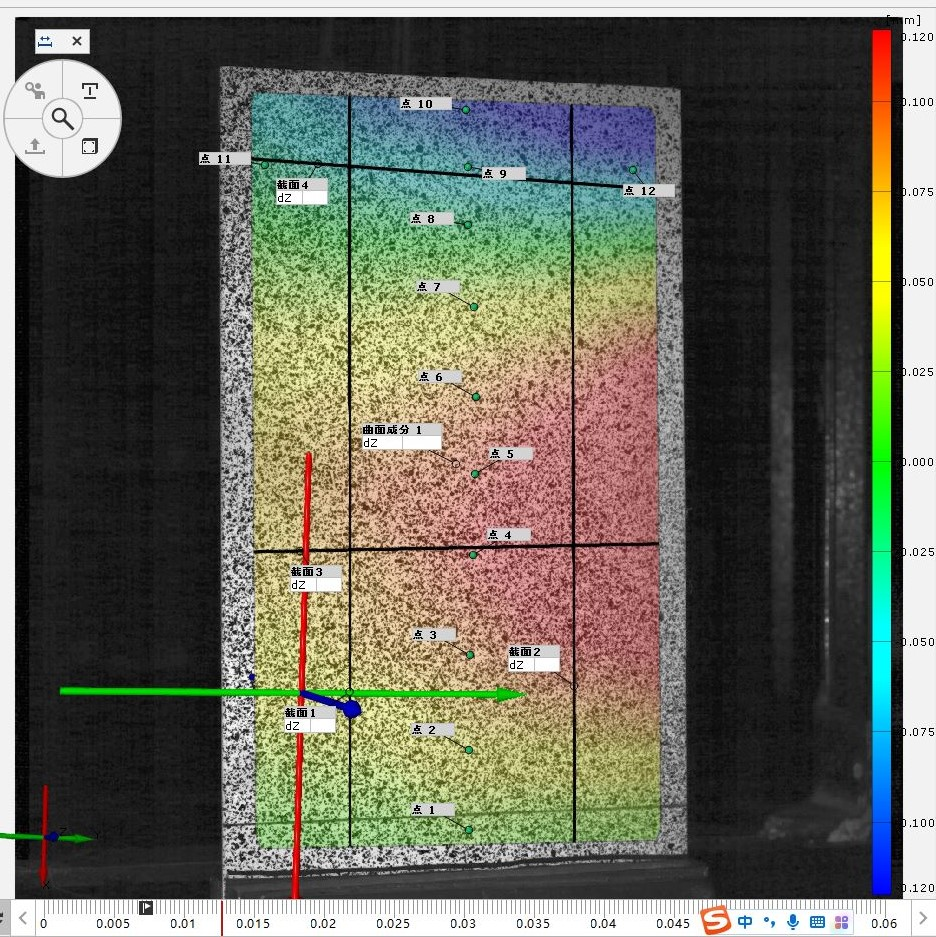
\includegraphics[width=\linewidth]{p09_img01.jpeg}}\hfill
\subcaptionbox{时刻2}[0.47\textwidth]{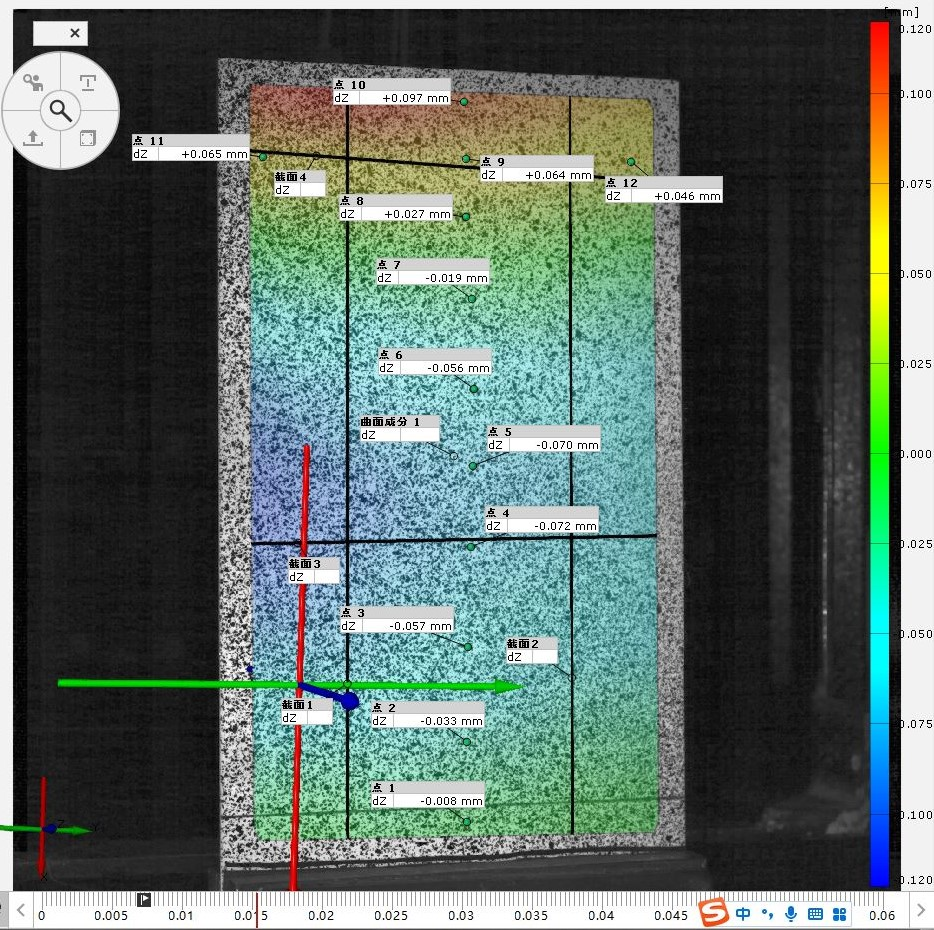
\includegraphics[width=\linewidth]{p09_img02.jpeg}}
\caption{二阶模态云图}
\label{fig:exp3-mode2-cloud}
\end{figure}

选取四个截面提取其沿 $z$ 坐标方向的位移信息，结果如图\ref{fig:exp3-mode2-section}所示。截面 1 与截面 2 沿纵向分布，用于观察弯曲模态；截面 3 与截面 4 沿横向分布，用于观察潜在的扭转模态。

\begin{figure}[H]
  \centering
  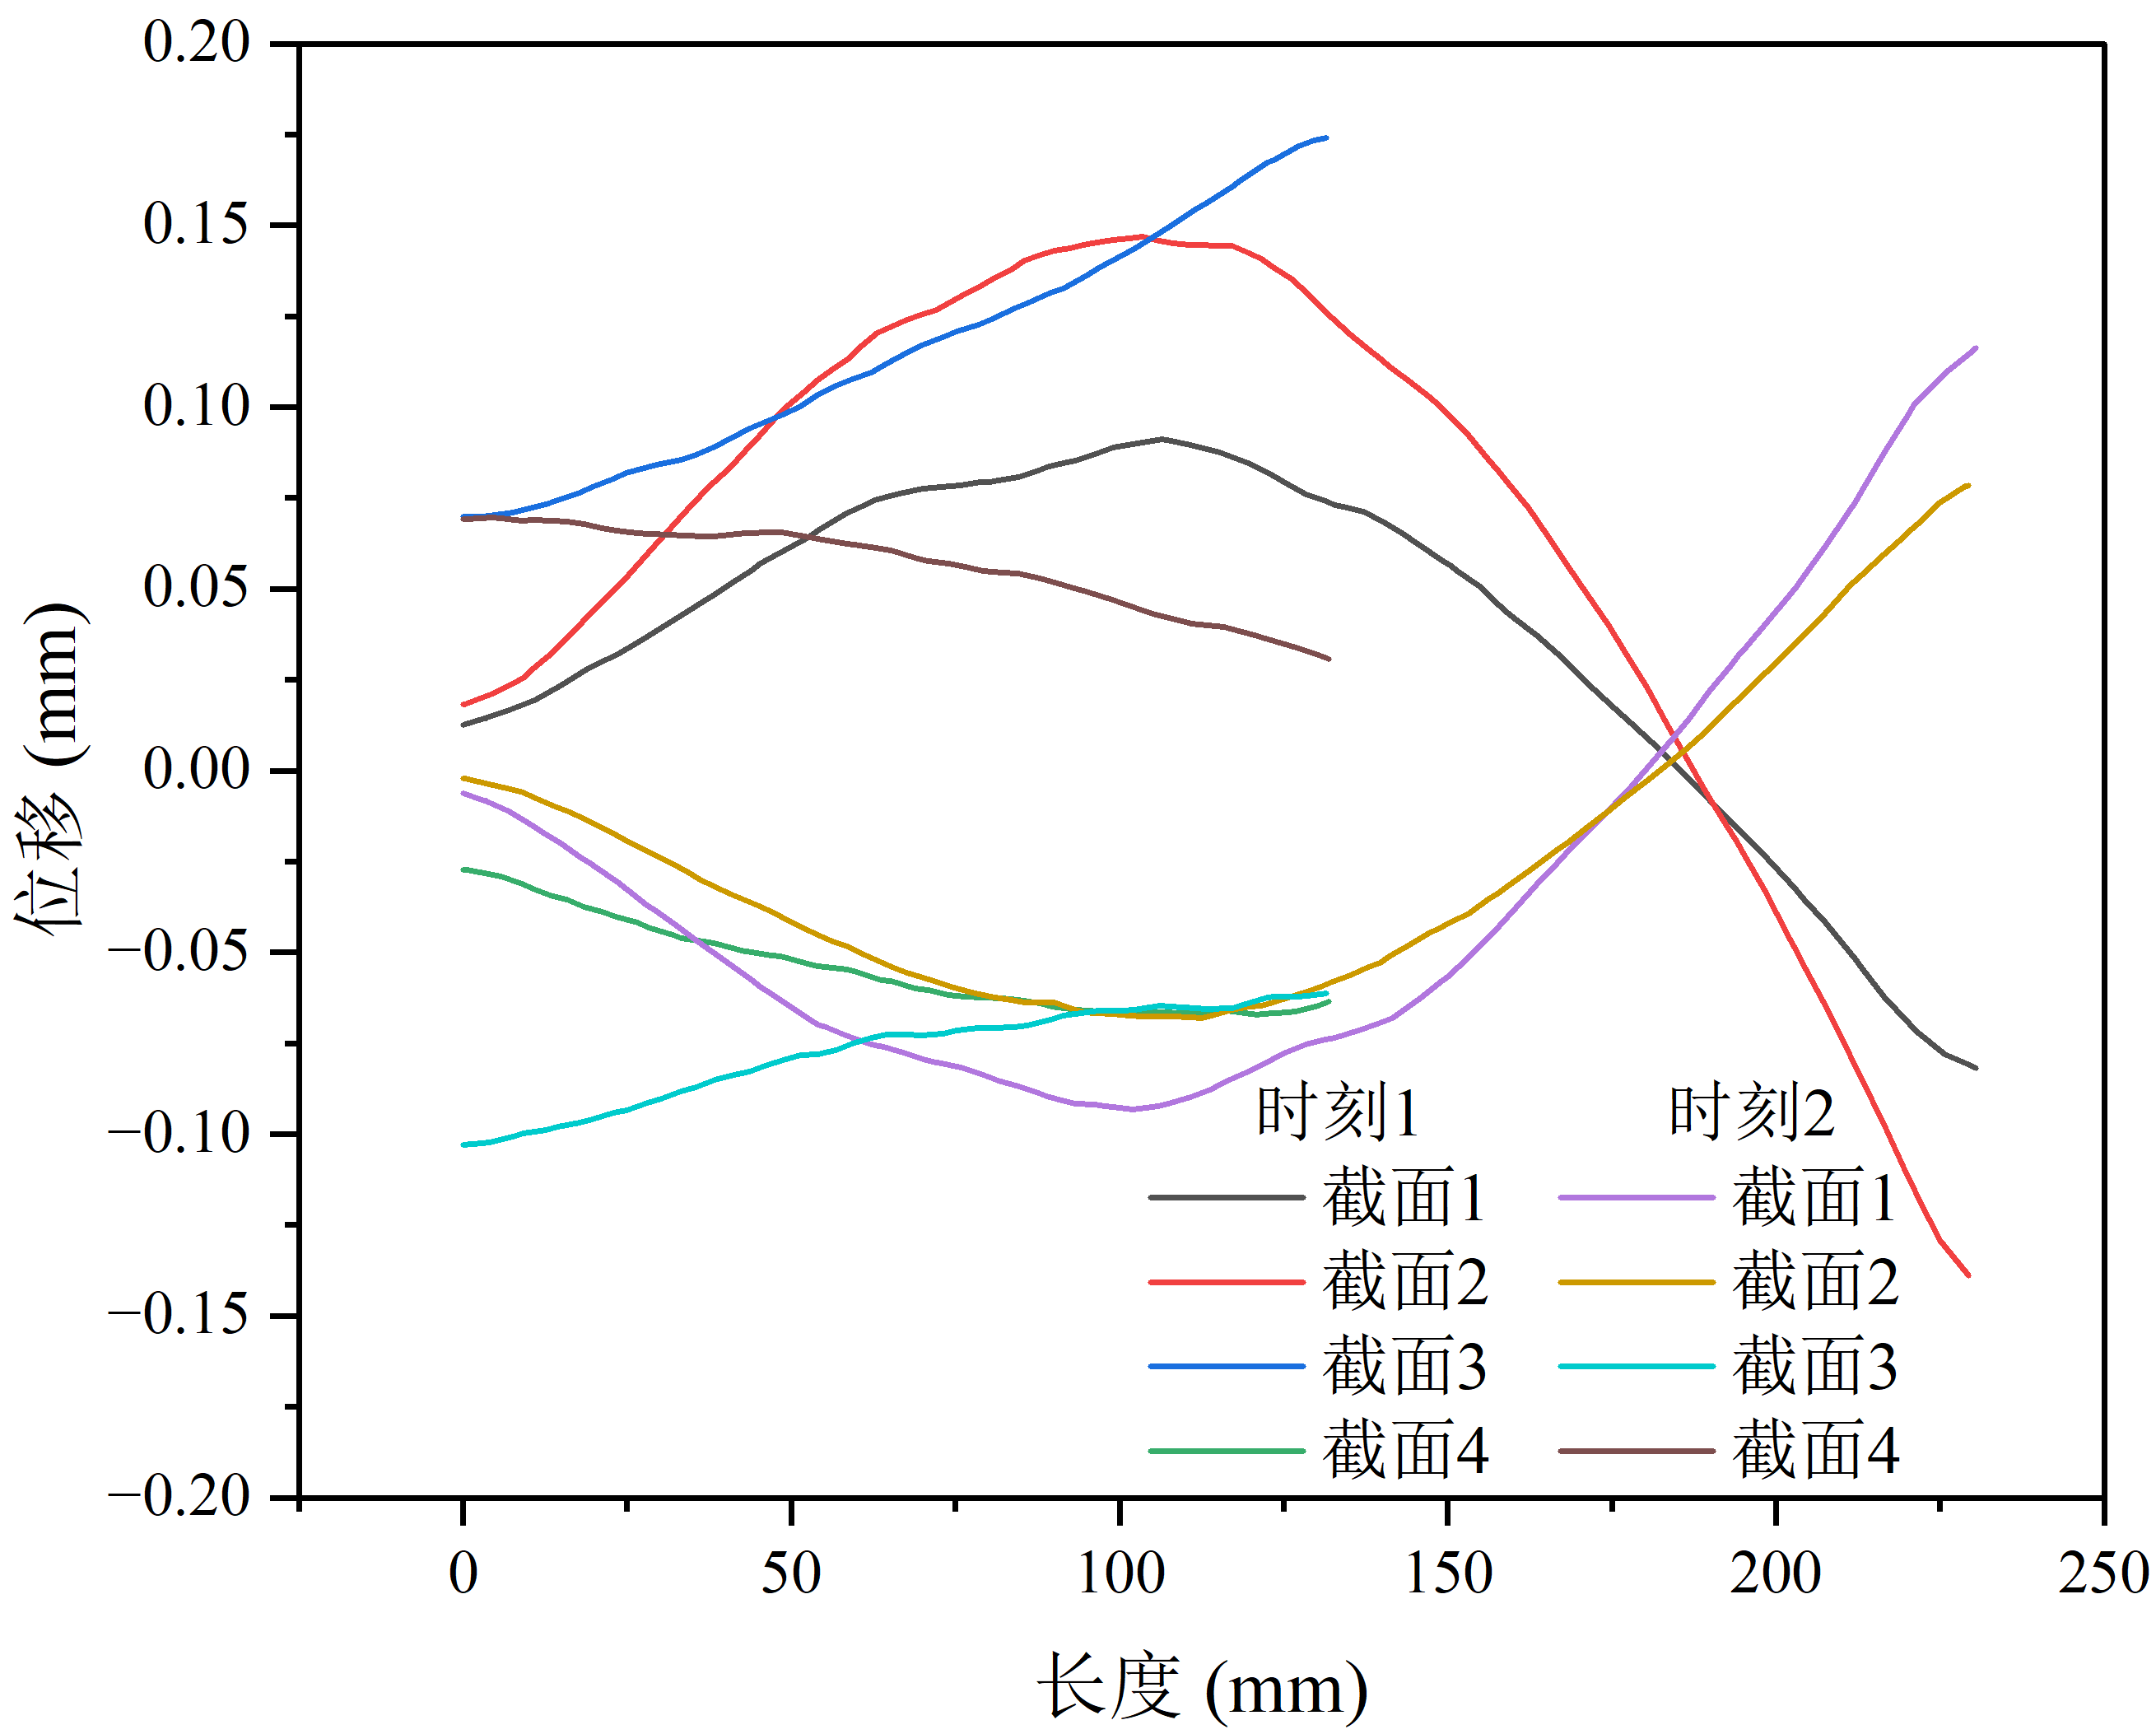
\includegraphics[width=0.7\textwidth]{p10_img01.png}
  \caption{二阶模态选取截面位移图}
  \label{fig:exp3-mode2-section}
\end{figure}
分析二阶模态的振幅分布和节点位置，比较各纵向及横向截面的位移曲线，并讨论激励位置是否引起扭转。
\answer

\subsection{点动态响应特征分析}
\subsubsection{一阶模态分析（23 Hz 激励）}
选取图\ref{fig:exp3-mode1-cloud}中的测量点进行点分析。1--5 号点沿固定方向纵向排列且大致位于板的中线上；2、6、7 号点近似处于同一水平位置；5、8、9 号点也近似处于同一水平位置。各测点位移随时间变化的曲线如图\ref{fig:exp3-mode1-points}所示。

\begin{figure}[H]
\centering
\subcaptionbox{测点组1}[0.31\textwidth]{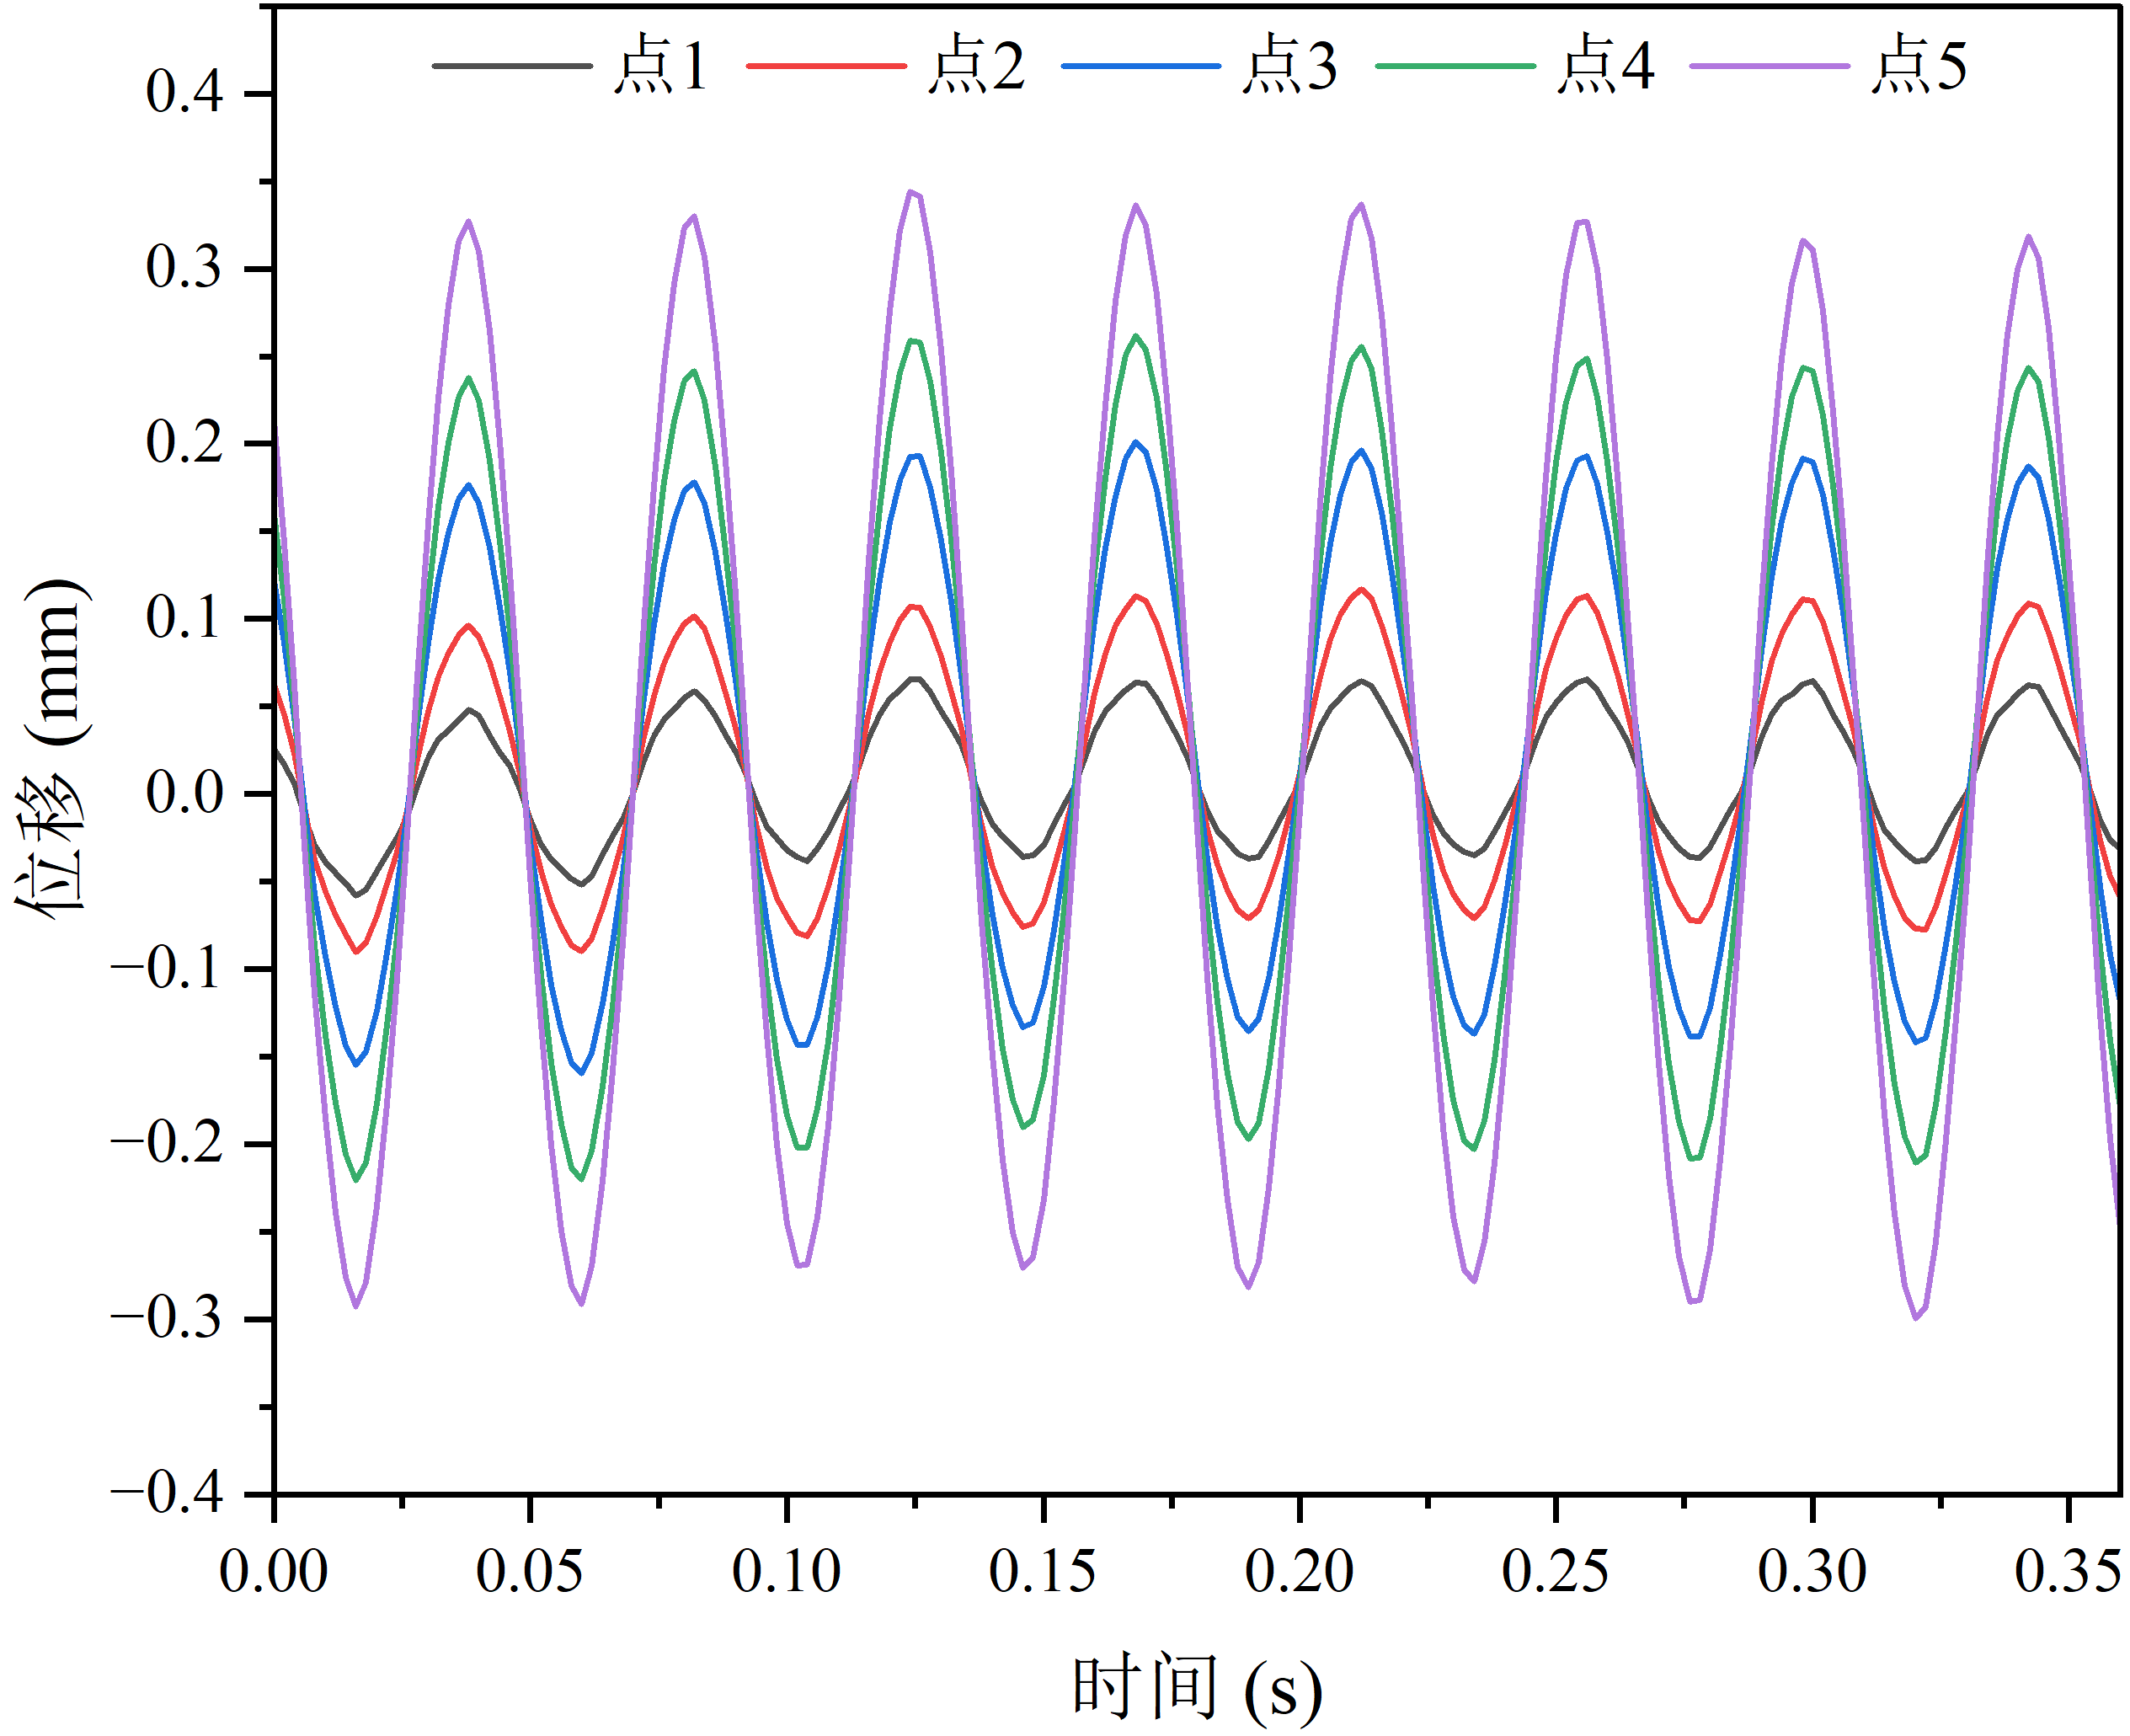
\includegraphics[width=\linewidth]{p10_img02.png}}\hfill
\subcaptionbox{测点组2}[0.31\textwidth]{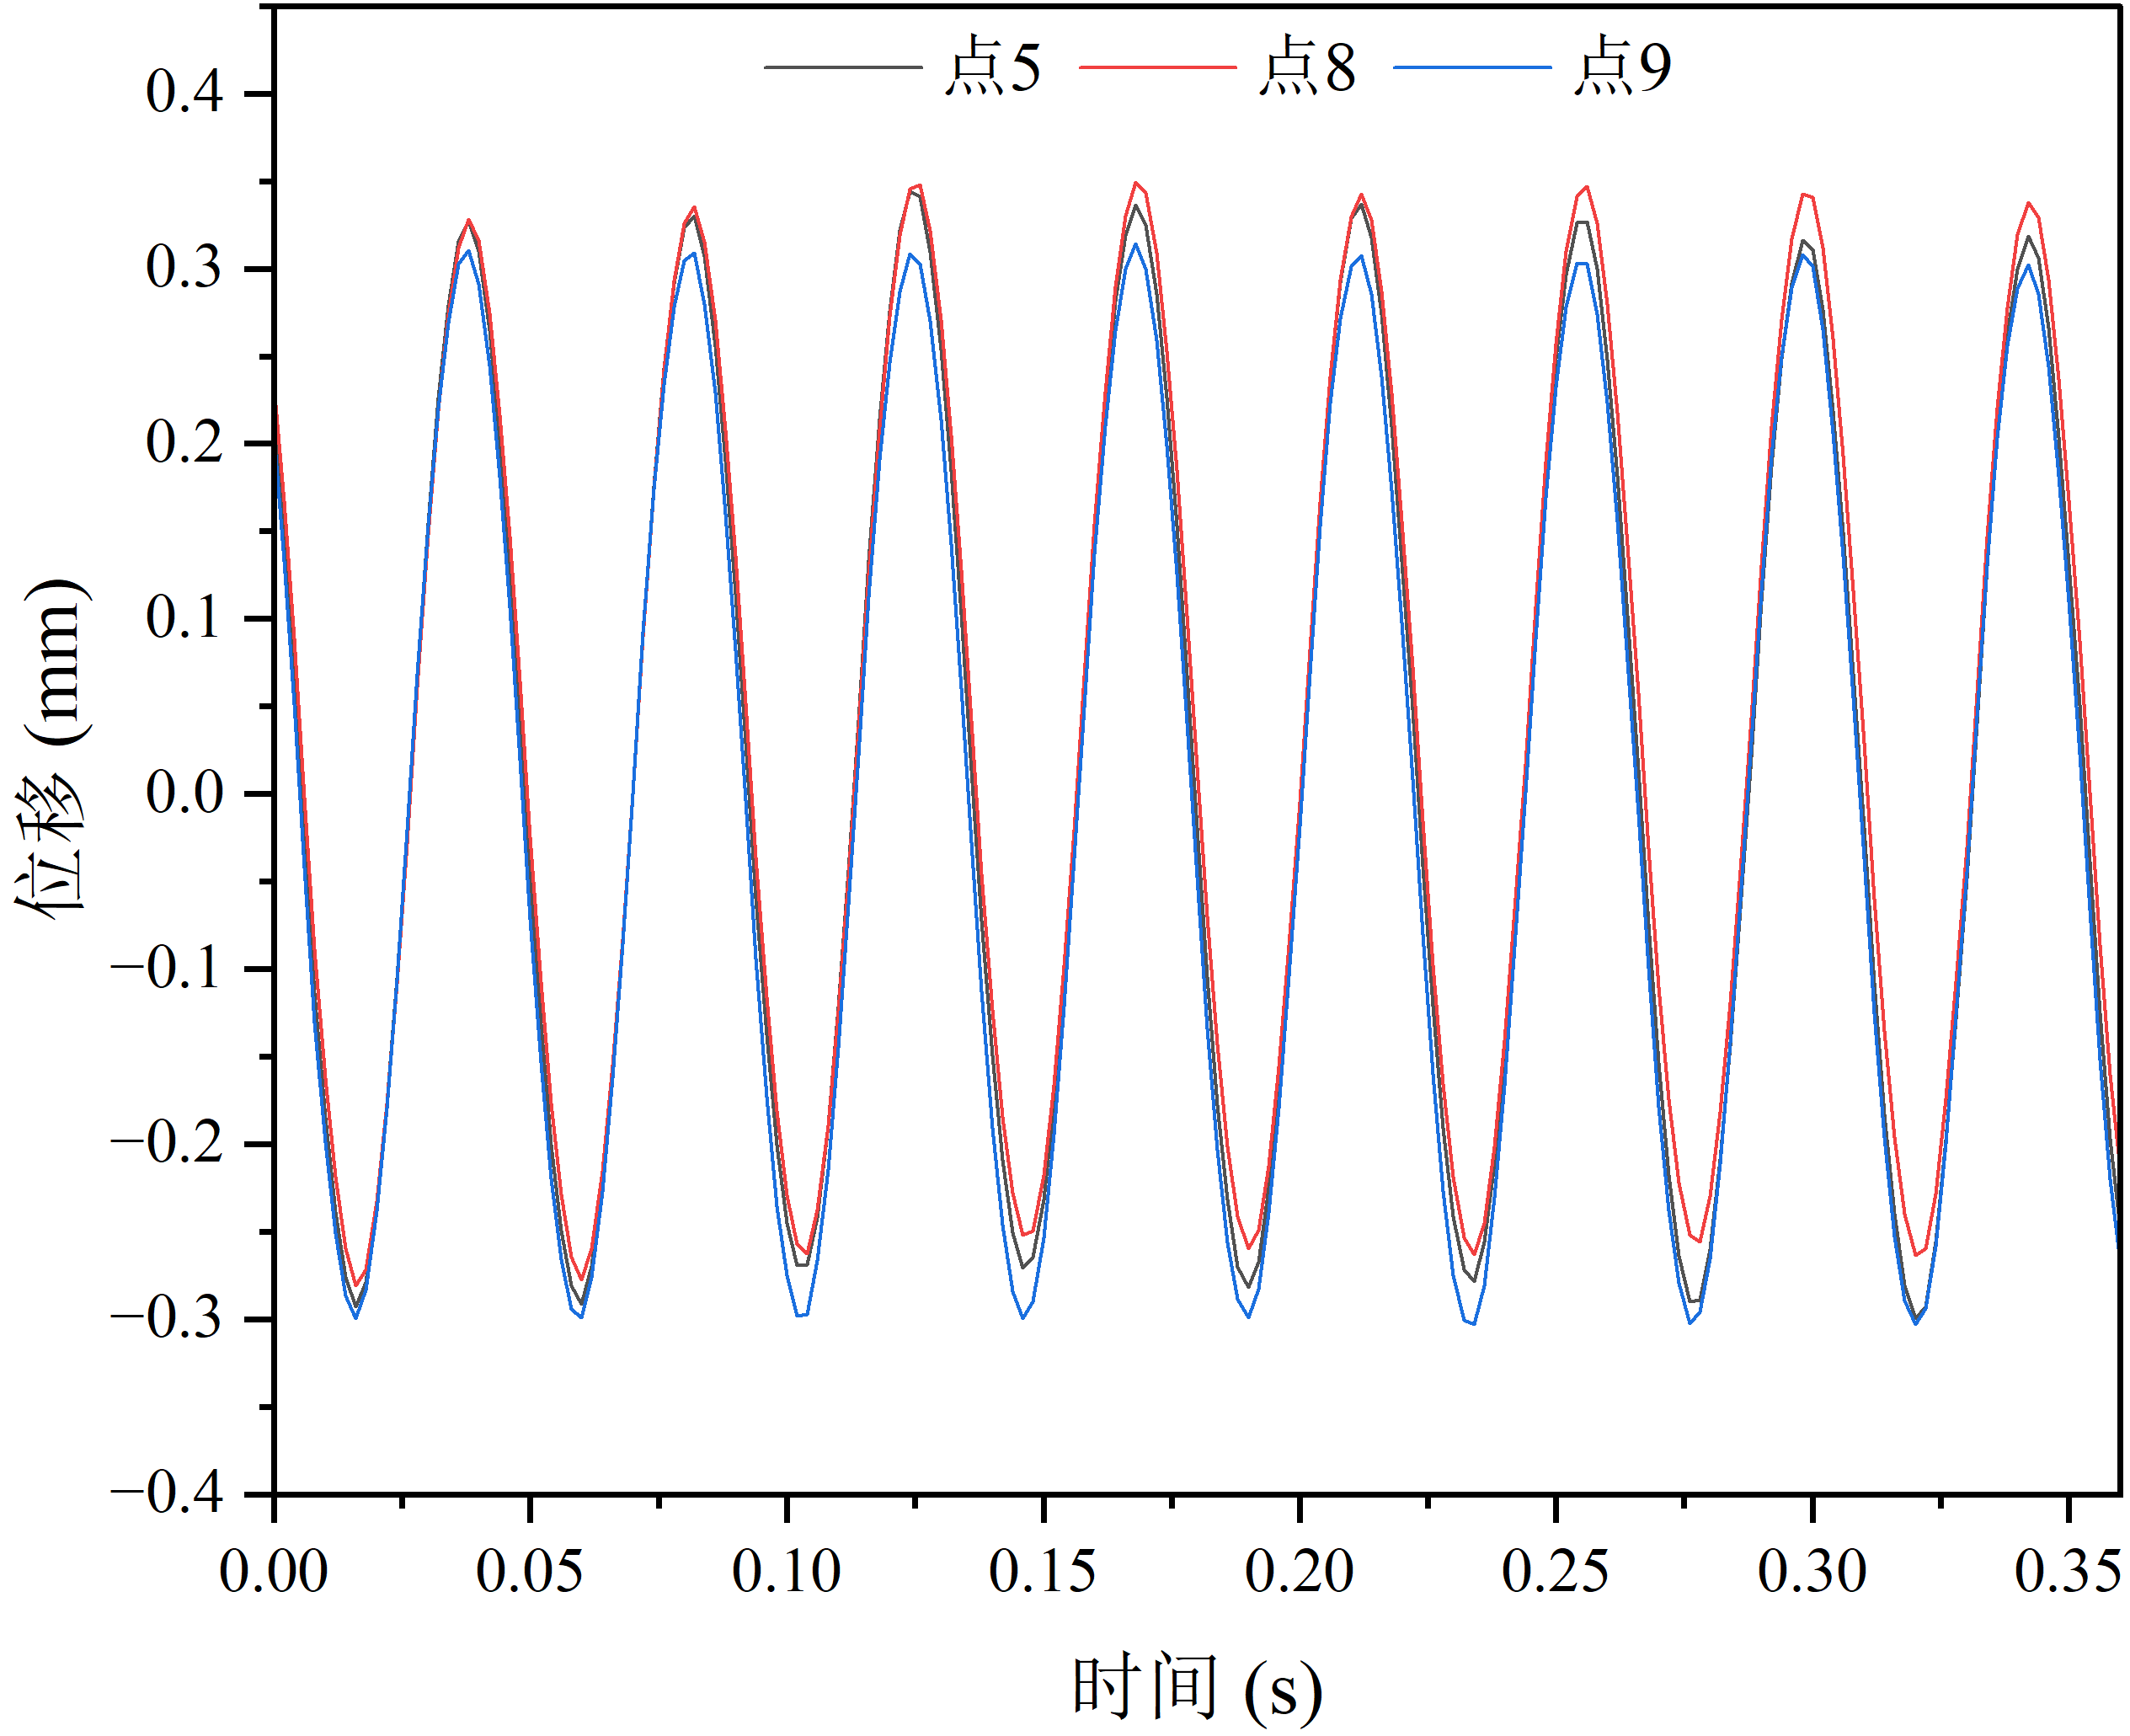
\includegraphics[width=\linewidth]{p10_img03.png}}\hfill
\subcaptionbox{测点组3}[0.31\textwidth]{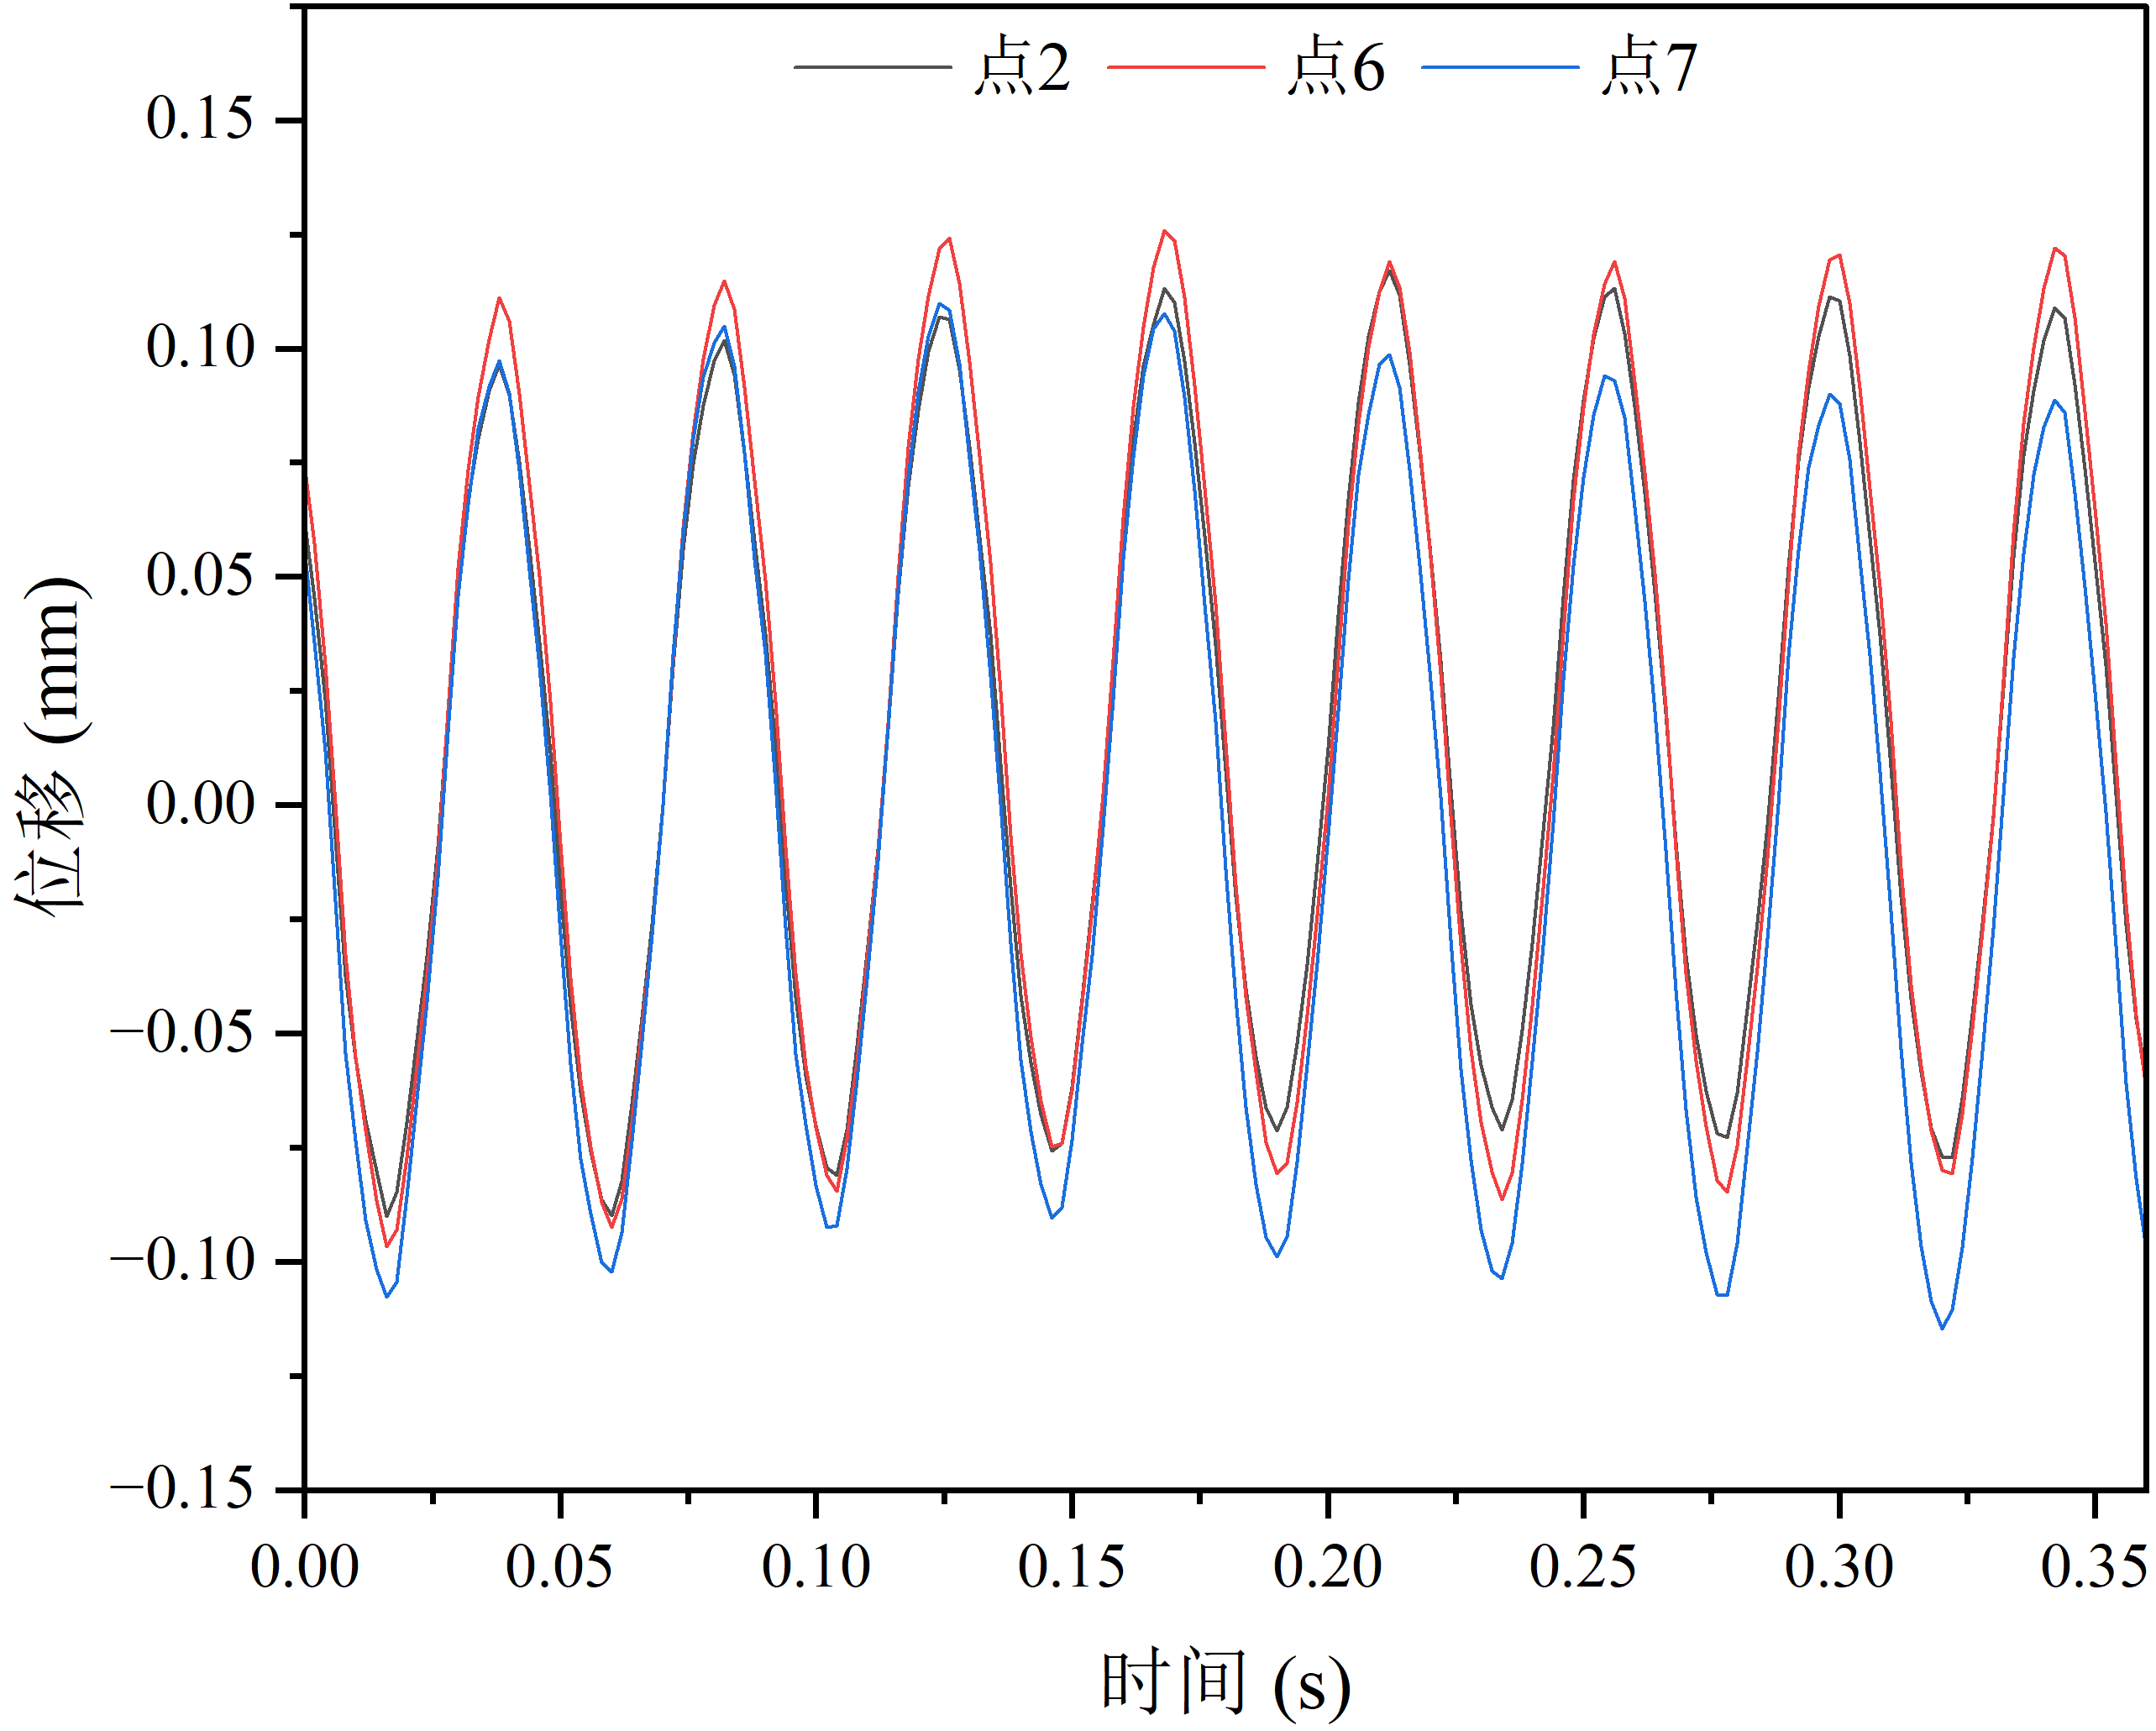
\includegraphics[width=\linewidth]{p10_img04.png}}
\caption{一阶模态选取点位移图}
\label{fig:exp3-mode1-points}
\end{figure}
分析各点振动频率、相位和振幅的关系，并与截面分析结果比较。
\answer

通过频率分析，在\blank[1.5cm] s 的采样时间内，样点经过\blank[1.2cm] 个周期，因此振动频率约为\blank[1.8cm] Hz；与施加的激振频率 23 Hz 比较，结果为\blank[3cm]。

\subsubsection{二阶模态分析（151 Hz 激励）}
选取图\ref{fig:exp3-mode2-cloud}中的测量点进行点分析。1--10 号点沿固定方向纵向排列且大致位于板的中线上，11、12 号点大致位于同一水平位置。各测点位移随时间变化的曲线如图\ref{fig:exp3-mode2-points}所示。

\begin{figure}[H]
\centering
\subcaptionbox{测点组1}[0.31\textwidth]{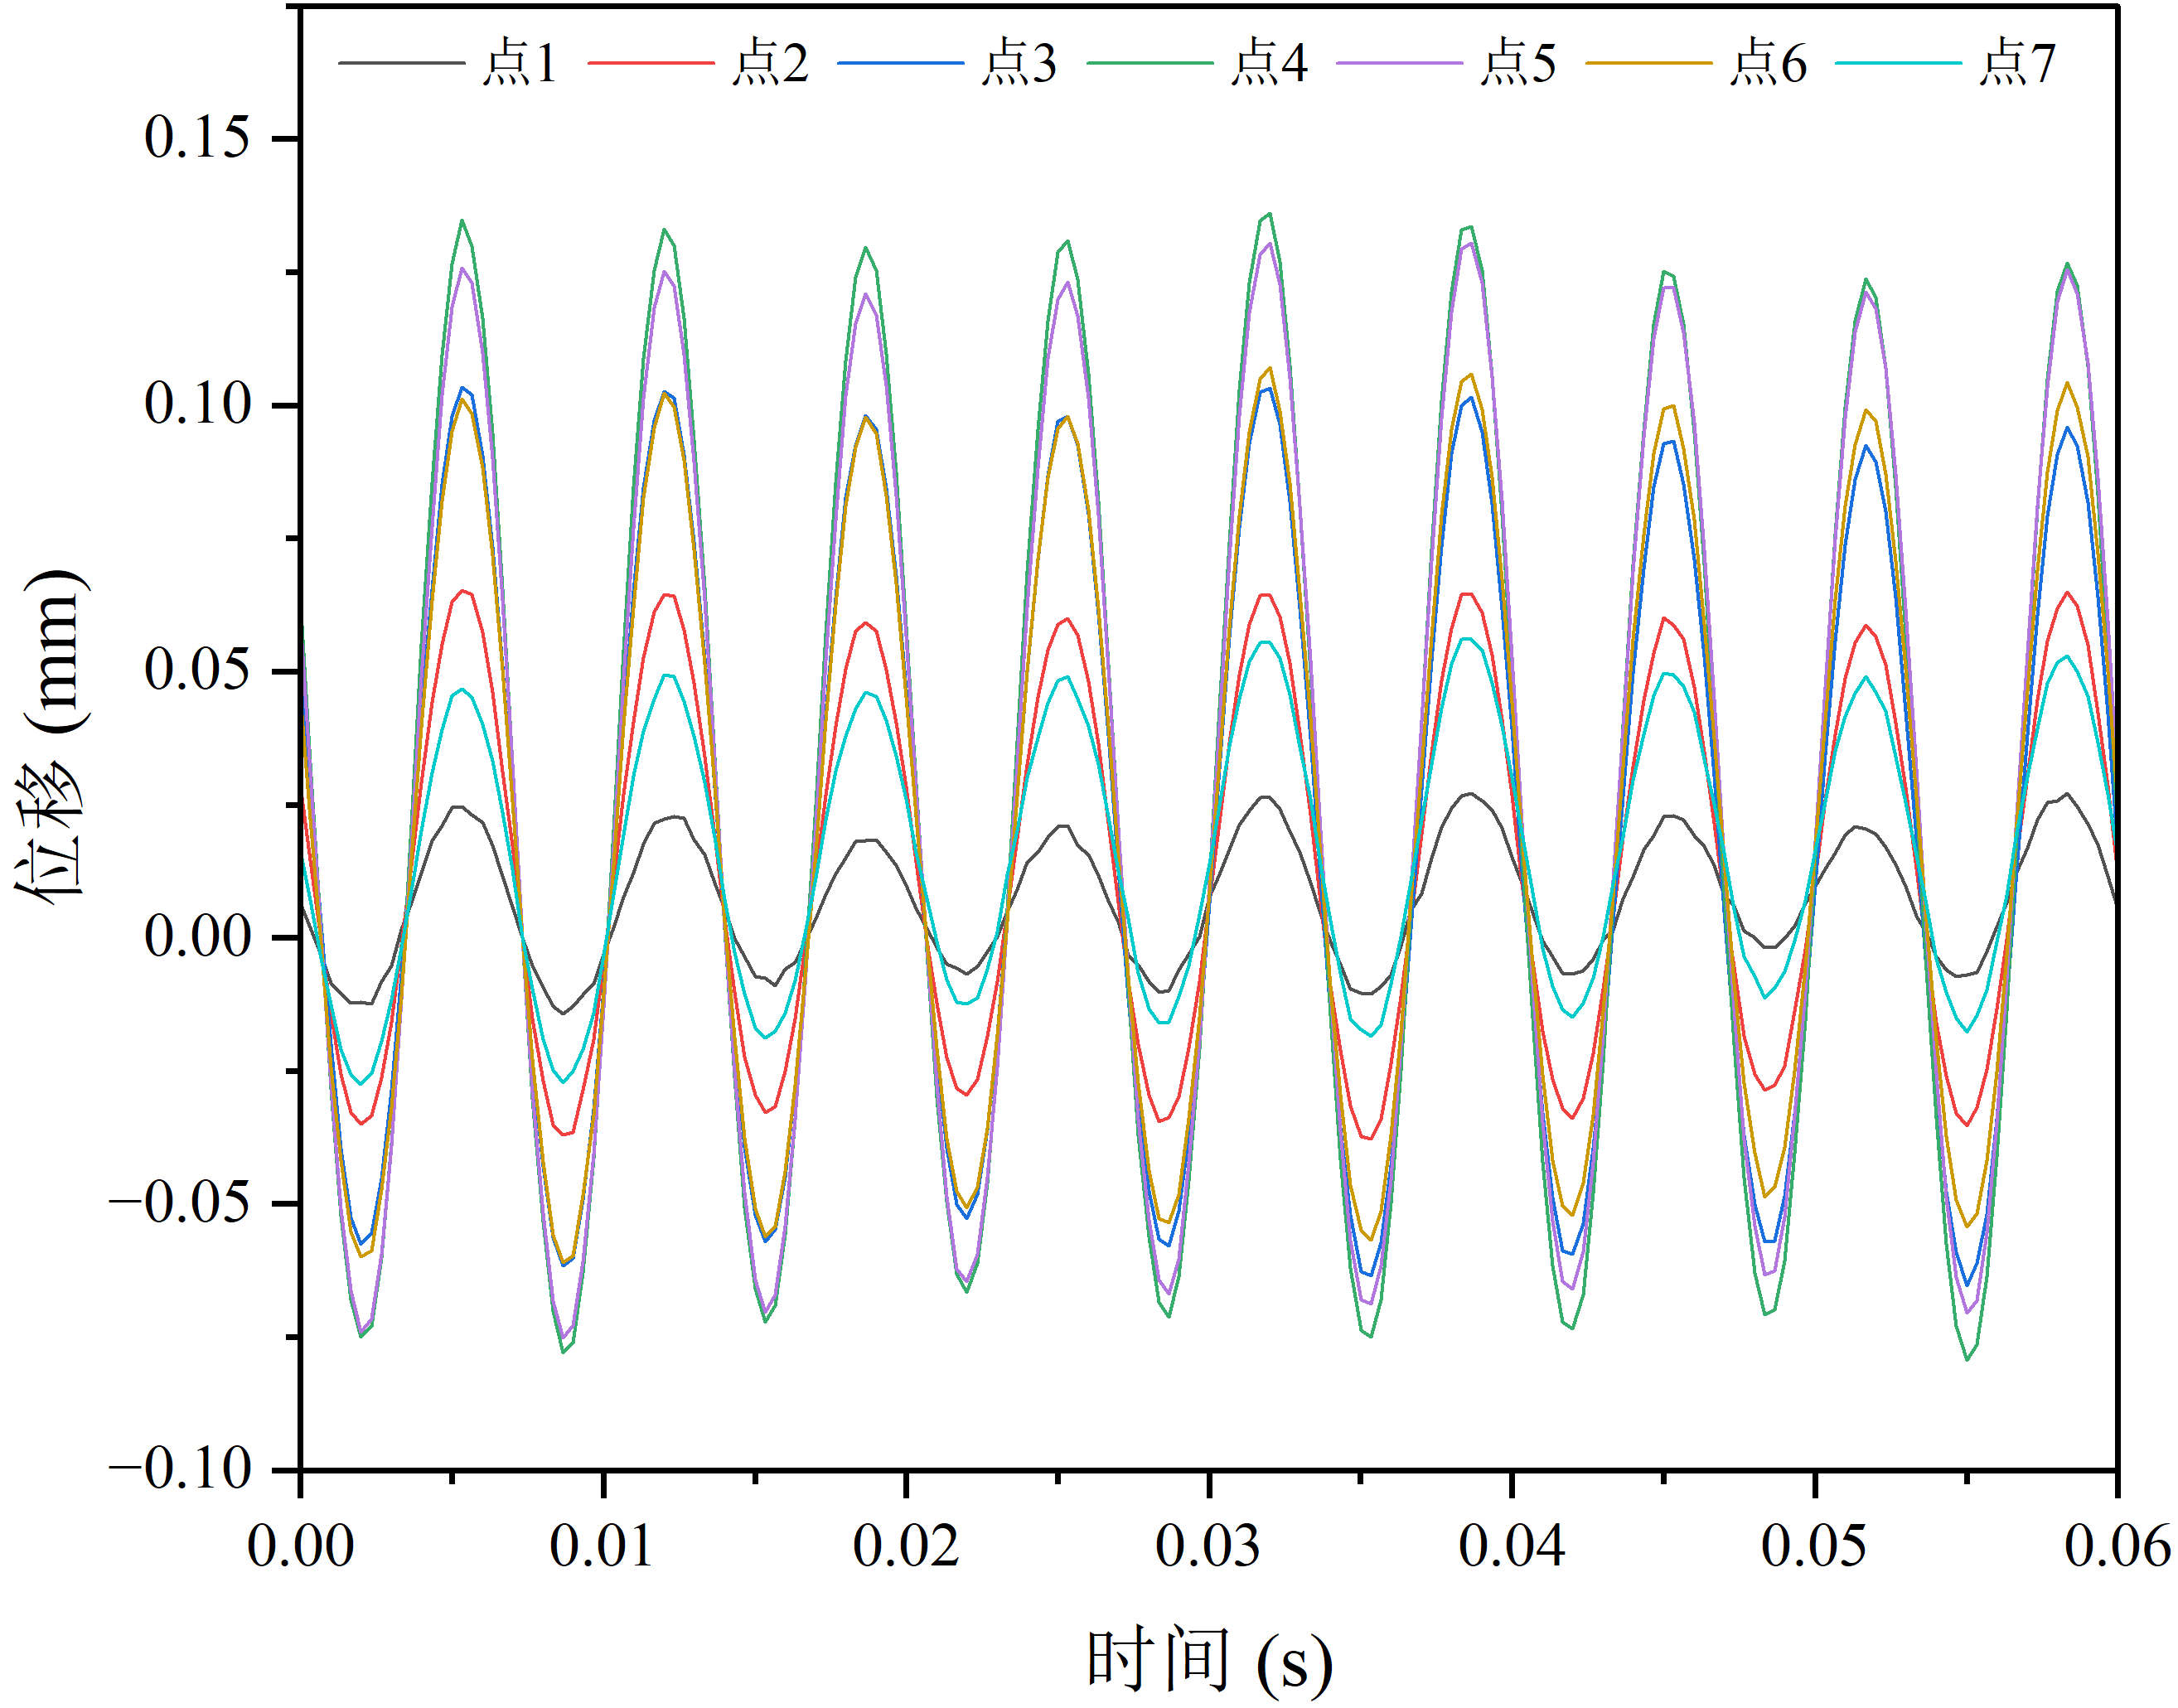
\includegraphics[width=\linewidth]{p11_img01.png}}\hfill
\subcaptionbox{测点组2}[0.31\textwidth]{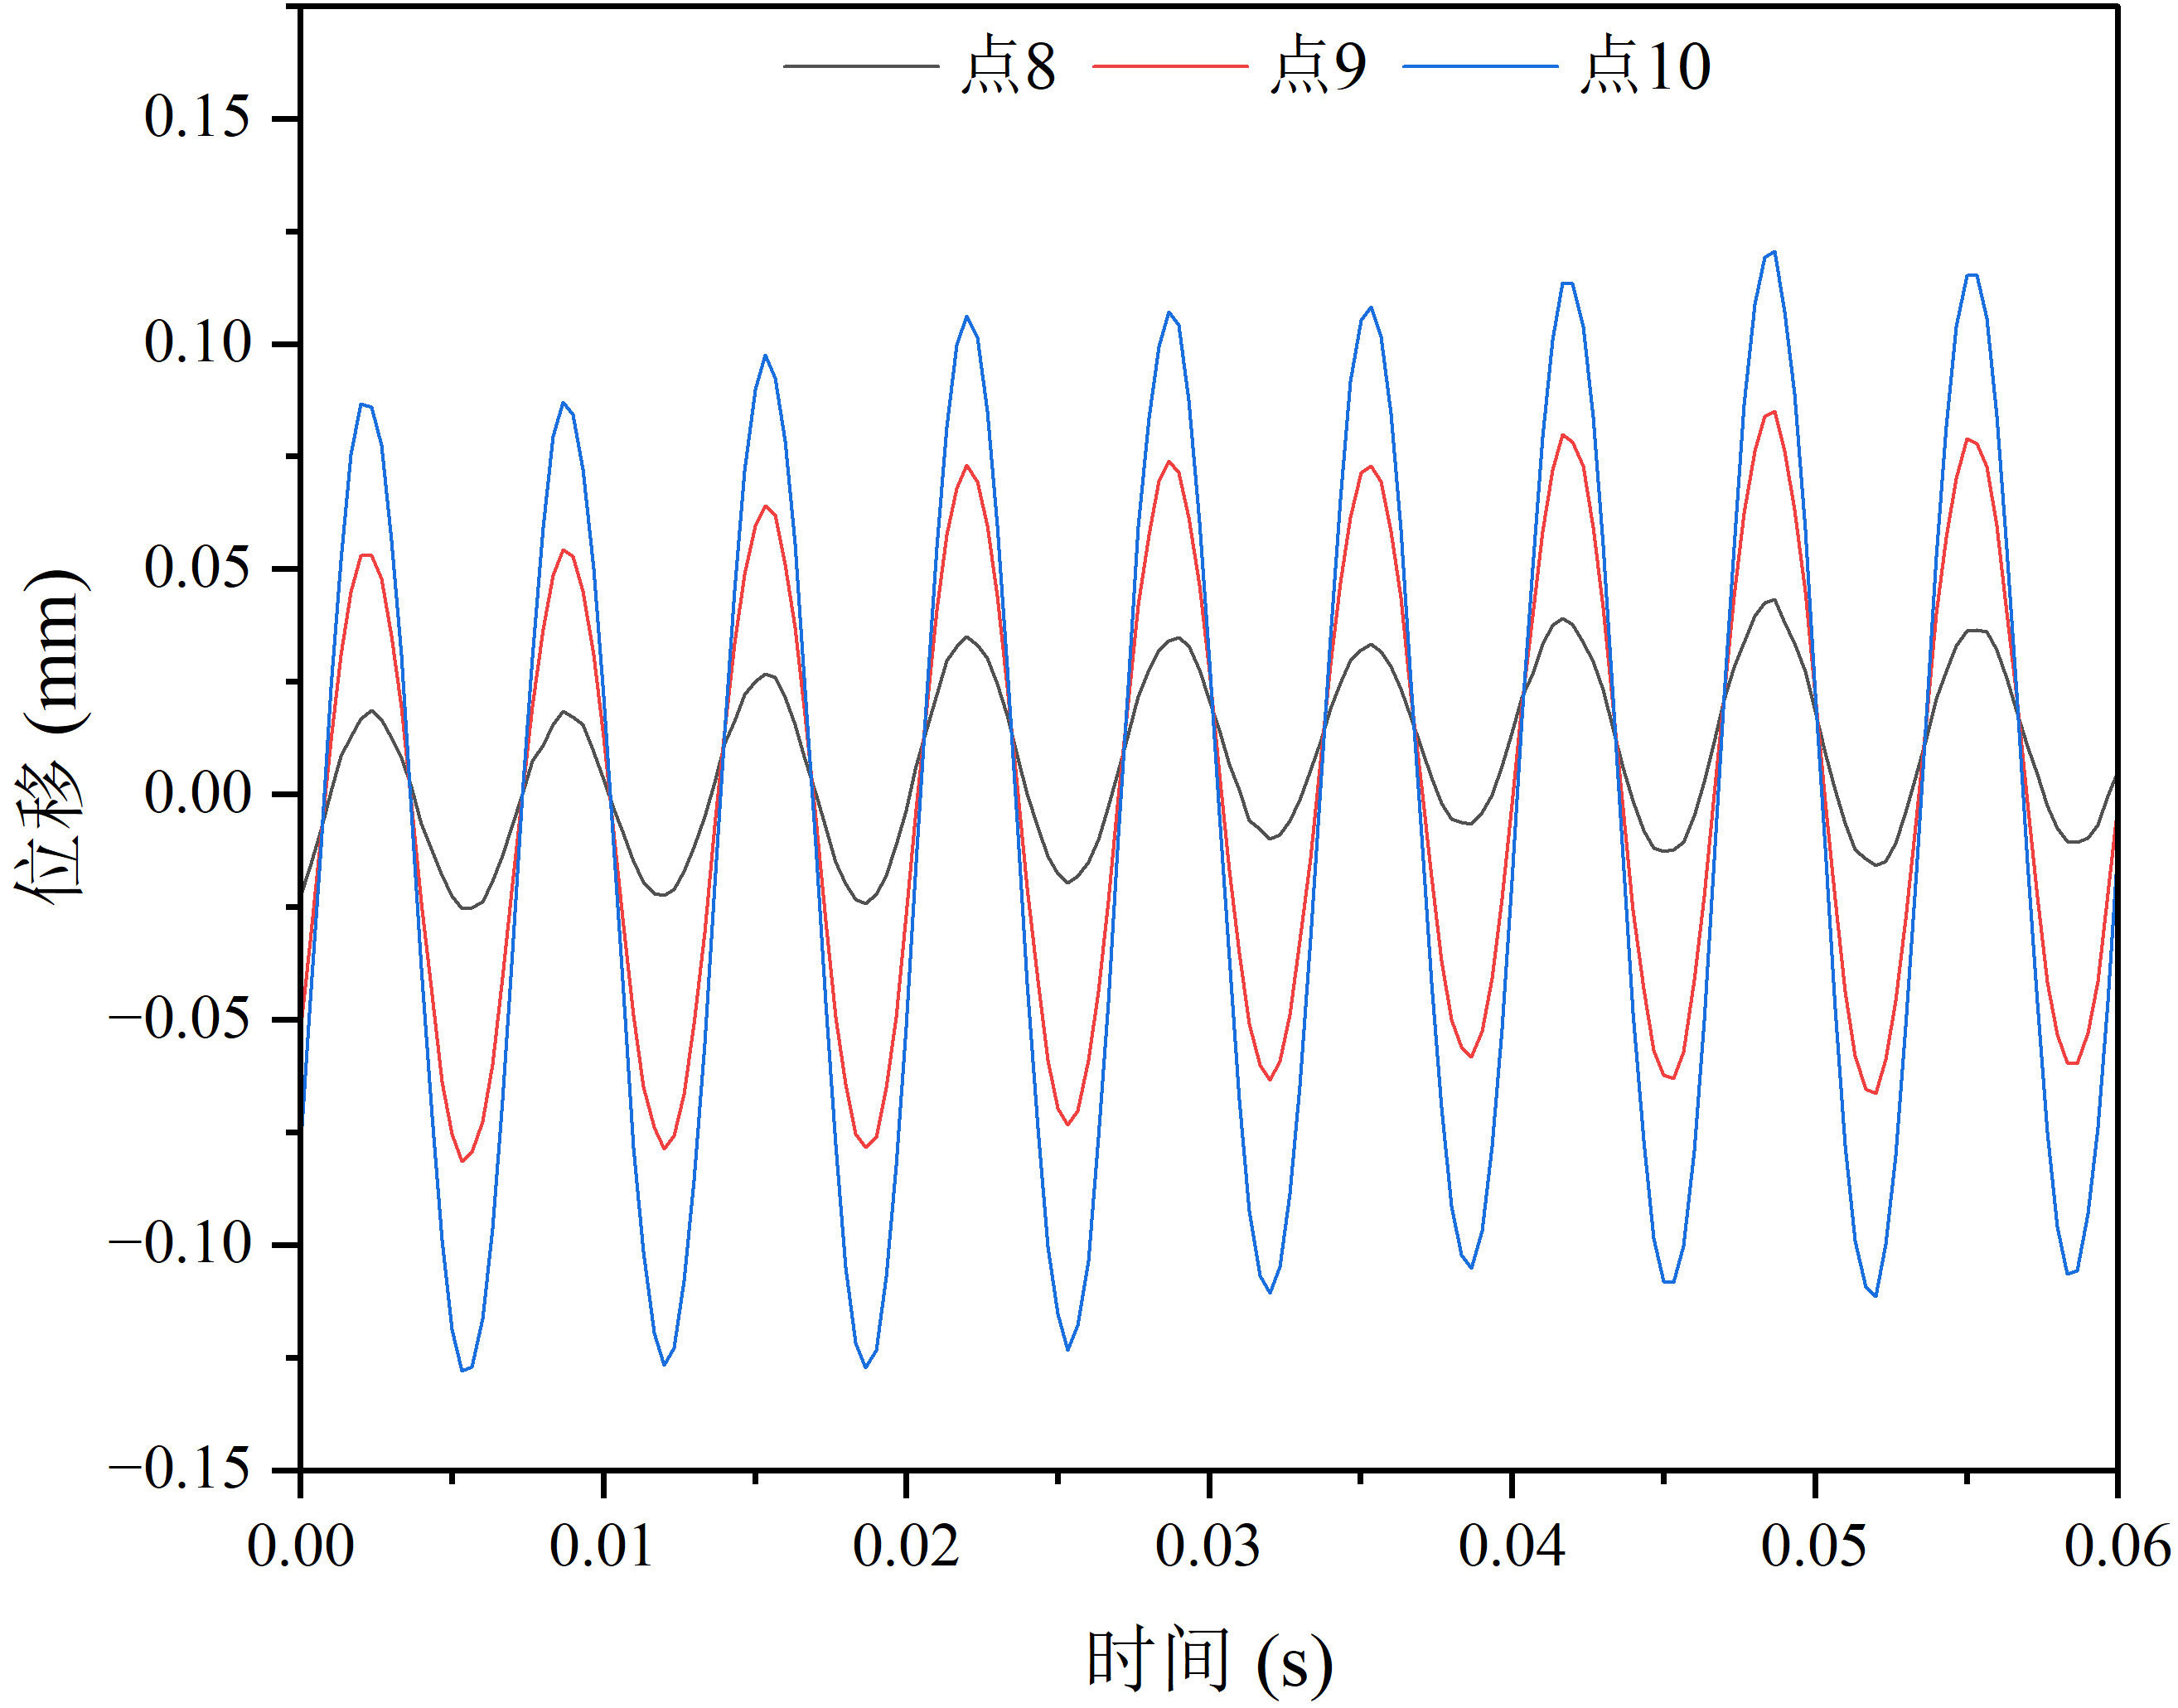
\includegraphics[width=\linewidth]{p11_img02.png}}\hfill
\subcaptionbox{测点组3}[0.31\textwidth]{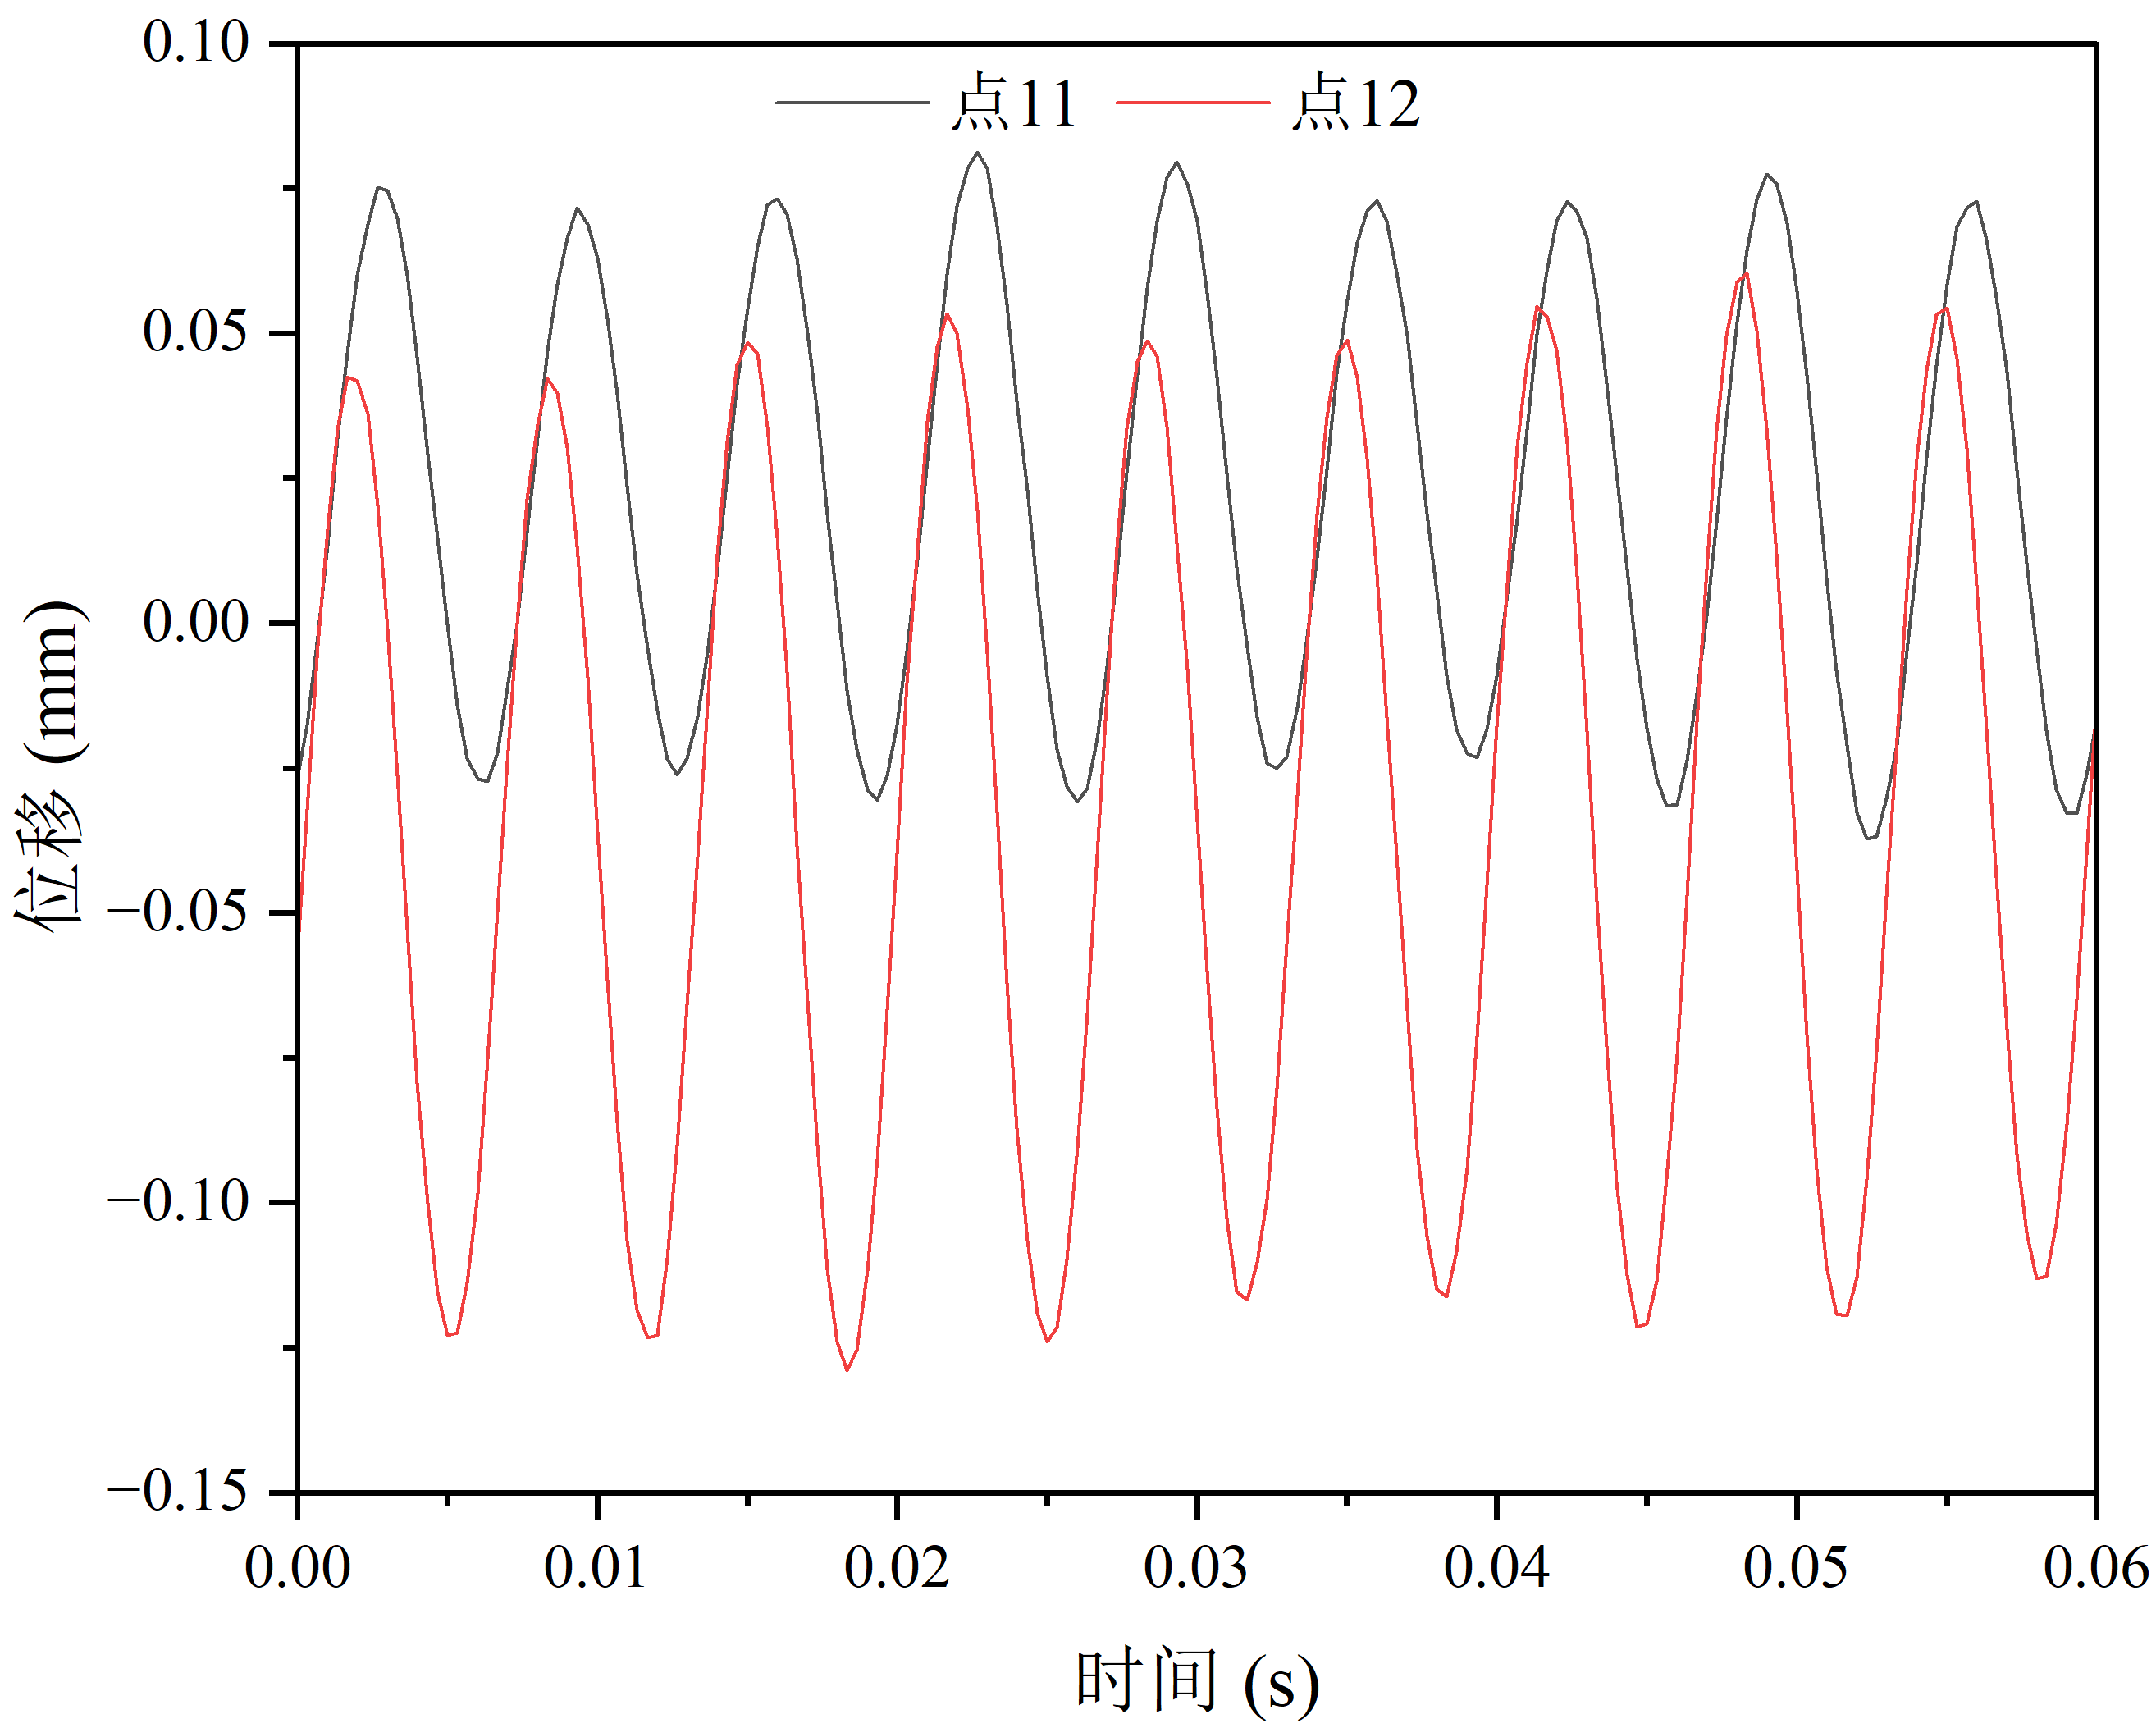
\includegraphics[width=\linewidth]{p11_img03.png}}
\caption{二阶模态选取点位移图}
\label{fig:exp3-mode2-points}
\end{figure}
分析各点振幅变化、节点两侧的相位关系，以及同一水平位置测点的差异是否与扭转模态有关。
\answer

通过频率分析，在\blank[1.5cm] s 的采样时间内，样点经过\blank[1.2cm] 个周期，因此振动频率约为\blank[1.8cm] Hz；与施加的激振频率 151 Hz 比较，结果为\blank[3cm]。

\section{数据误差分析与提高精度的方法}
\begin{enumerate}
  \item 比较低频和高频激励下的模态识别结果，分析各点振动频率是否接近激励频率、振幅变化是否符合预期，以及是否出现混合扭转模态。
  \item 相机标定过程可能存在一定误差，会影响图像和位移测量的准确性。
  \item 在图像处理过程中，选择曲面成分时应尽可能选取较大区域，以采集更多位置信息，从而降低误差的影响。
  \item 激振器的位置可能对模态测量结果产生影响，应确保激振器的作用方向经过板的弯曲中心，以最大限度消除扭转效应。
  \item 若板固支端存在松动或激振器与板之间接触不紧密，可能引入误差。为了更准确地测量板的弯曲模态并减少扭转模态的影响，应改善固支端的夹持均匀性与牢固性。
\end{enumerate}
结合本组图像和曲线补充误差分析。
\answer

\end{document}
